\documentclass[12pt]{article}
\usepackage[utf8]{inputenc}
\usepackage[brazil]{babel}
\usepackage{graphicx}
\usepackage{listings}
\usepackage{xcolor}
\usepackage{amsmath}
\usepackage{geometry}
\usepackage{float}
\lstset{showstringspaces=false}
\geometry{a4paper, margin=2.5cm}

% Numeracao das subsections como 1.a), 1.b), 2.a), ...
\renewcommand{\thesubsection}{\thesection.\alph{subsection})}

% Configuração para códigos Matlab
\lstset{
    language=Matlab,
    basicstyle=\ttfamily\small,
    keywordstyle=\color{blue},
    stringstyle=\color{red},
    commentstyle=\color{green!60!black},
    numbers=left,
    numberstyle=\tiny,
    stepnumber=1,
    frame=single,
    breaklines=true,
    extendedchars=true,
    literate={á}{{\'a}}1 {ã}{{\~a}}1 {õ}{{\~o}}1 {é}{{\'e}}1 {í}{{\'i}}1 {ó}{{\'o}}1 {ú}{{\'u}}1 {ç}{{\c{c}}}1
}

\title{Relatório: Prática 3 - Amostragem e Quantização \\ \large Análise de Sistemas Lineares - UTFPR}
\author{Leonardo Pereira Shibata \\ Sergio Roncato Maccari}
\date{Abril de 2026}

\begin{document}

\begin{titlepage}
    \begin{center}
        \Large \textbf{UNIVERSIDADE TECNOLÓGICA FEDERAL DO PARANÁ} \\
        \Large \textbf{CURSO DE ENGENHARIA DE COMPUTAÇÃO} \\
        \large ELEQ30 - Análise de Sistemas Lineares \\
        \large Professor César Janeczko \\
        \vspace{5cm}
        \huge \textbf{Relatório: Prática 3} \\
        \large \textbf{Amostragem e Quantização} \\
        \vspace{1.5cm}
        \Large \textbf{Disciplina: Análise de Sistemas Lineares} \\
        \vspace{4cm}
        \Large Leonardo Pereira Shibata \\
        \Large Sergio Roncato Maccari \\
        \vfill
        \Large Curitiba, Abril de 2026
    \end{center}
\end{titlepage}

\section{Amostragem e Quantização}

\subsection{Faça a função \texttt{quantiza} a partir da expressão $x_{aM} = \mathrm{floor}(x/2^{8-M})\cdot 2^{8-M}$ e salve como arquivo \texttt{quantiza.m}}

A função recebe dois parâmetros de entrada ($x$, $M$) e devolve uma resposta $X_{am}$, conforme o enunciado.

\begin{lstlisting}
function [Xam] = quantiza(x, M)
    Xam = floor(x / 2^(8-M)) * 2^(8-M);
end
\end{lstlisting}

Internamente, a função divide o sinal pelo passo de quantização $\Delta = 2^{8-M}$, aplica \texttt{floor} para travar no nível inferior, e remultiplica por $\Delta$. O efeito prático é mapear cada amostra para o múltiplo inteiro de $\Delta$ imediatamente abaixo dela, gerando uma versão de $x$ com apenas $2^M$ valores possíveis dentro da faixa de 8 bits.

\subsection{Execute o exemplo. Compare os sinais e tire suas conclusões}

\begin{lstlisting}
s10 = senoide(128, -127, 2, 1000); % "continuo" 10Hz, 1000 pontos
s10amostrado = senoide(128, -127, 2, 20); % sinal amostrado (20 amostras)
indice = 1:50:1000; % vetor para esticar 20 sobre 1000

plot(s10, 'b', 'LineWidth', 1.3); hold on;
plot(indice, s10amostrado, 'o-r', 'LineWidth', 1.3);
stairs(indice, quantiza(s10amostrado, 2), 'm', 'LineWidth', 1.3);
title('quantizacao 2 bits FLOOR'); grid on;
\end{lstlisting}

\begin{figure}[H]
    \centering
    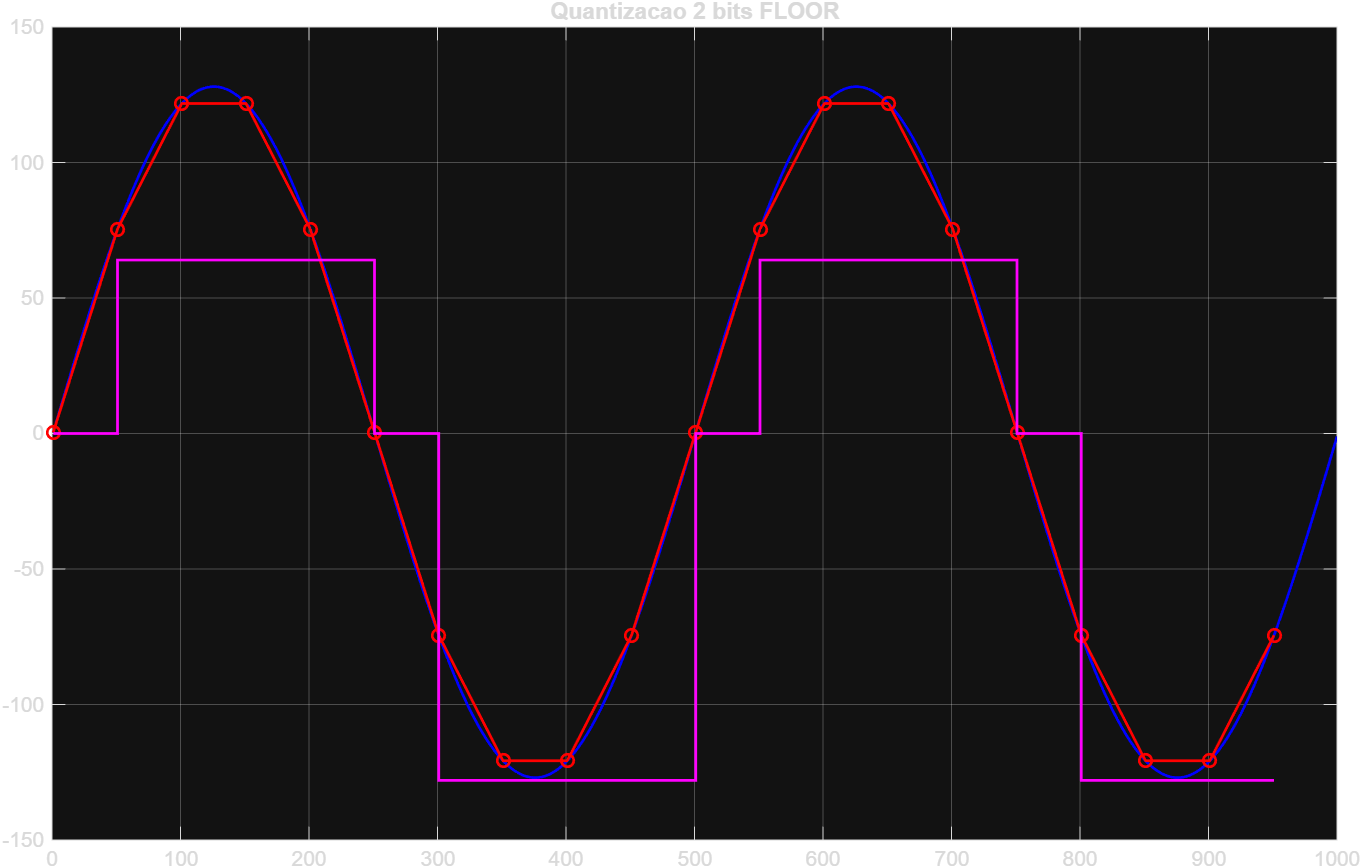
\includegraphics[width=0.85\textwidth]{imgs/q1b_floor_2bits.png}
    \caption{Sinal contínuo (azul), amostrado (vermelho) e quantizado em 2 bits com \texttt{floor} (magenta).}
\end{figure}

\textbf{Conclusões:} Com $M=2$ temos $2^{2}=4$ níveis utilizáveis dentro da faixa nominal de 8 bits e passo de quantização $\Delta = 2^{8-2} = 64$. Os patamares disponíveis são $\{-128,\,-64,\,0,\,64\}$, ou seja, apenas quatro degraus para representar uma onda que oscila entre $-127$ e $128$. A perda de informação é severa: a curva degrau magenta praticamente não acompanha a senoide, ficando restrita a alguns intervalos planos. Como o \texttt{floor} sempre arredonda para baixo, todo patamar fica deslocado em relação ao valor real da senoide, gerando um erro sistemático negativo de até $-\Delta = -64$. Esse \emph{bias} é particularmente prejudicial porque desloca toda a forma de onda para baixo, alterando inclusive a média (componente DC) do sinal — o que em aplicações de áudio ou medidas físicas pode ser inaceitável. Há ainda um efeito de saturação assimétrica na crista positiva, já que o nível $128$ não está disponível como degrau intermediário (cai sobre $64$).

\subsection{Trocar o \texttt{floor} por \texttt{round}. Qual a diferença?}

\begin{lstlisting}
function [Xam] = quantiza(x, M)
    Xam = round(x / 2^(8-M)) * 2^(8-M);
end
\end{lstlisting}

\begin{figure}[H]
    \centering
    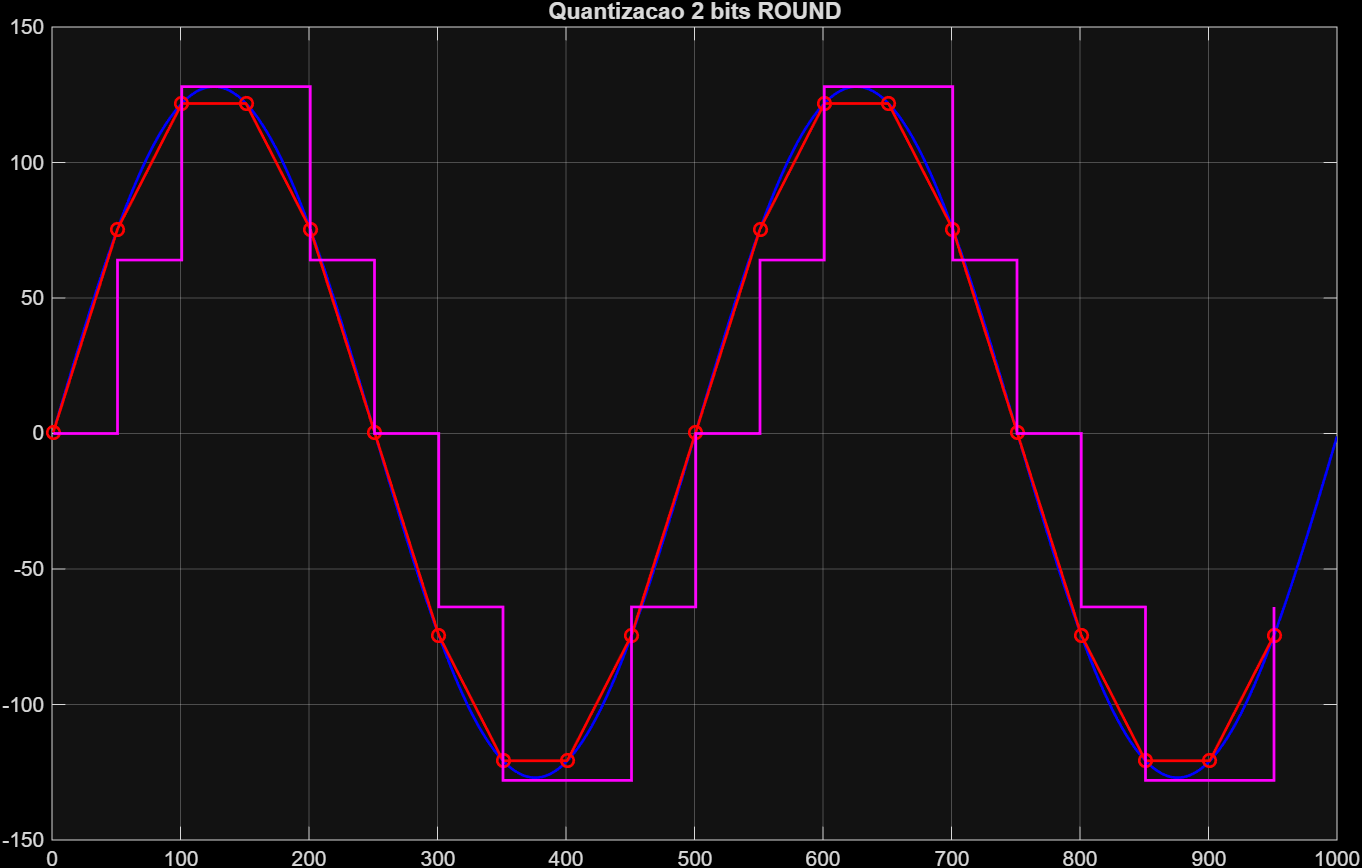
\includegraphics[width=0.85\textwidth]{imgs/q1c_round_2bits.png}
    \caption{Quantização em 2 bits utilizando \texttt{round}.}
\end{figure}

\textbf{Diferença:} A diferença concentra-se principalmente nos picos e vales do sinal. Enquanto o \texttt{floor} produz erro $e \in [-\Delta,\,0]$ (apenas negativo), o \texttt{round} produz erro $e \in [-\Delta/2,\,+\Delta/2]$, distribuído simetricamente. Em termos práticos, a magnitude máxima do erro cai pela metade, e o \emph{bias} sistemático do sinal vai a zero — a média do sinal é preservada. É como ganhar quase um bit de resolução efetiva apenas pela escolha do método de arredondamento. Visualmente, os patamares do degrau ``abraçam'' a senoide alternando acima e abaixo, em vez de ficar sempre abaixo. Em conversores ADC reais é prática comum adicionar meio passo antes de aplicar \texttt{floor} (truncamento) justamente para reproduzir o comportamento de \texttt{round} sem custo de hardware adicional.

\subsection{Repetir tudo para 5 bits. Compare o número de degraus para 2 e 5 bits. Tire as suas conclusões}

Com $M=5$ o passo de quantização cai para $\Delta = 2^{8-5}=8$ e passamos a ter $2^{5}=32$ níveis, o que reduz fortemente o erro de quantização.

\begin{figure}[H]
    \centering
    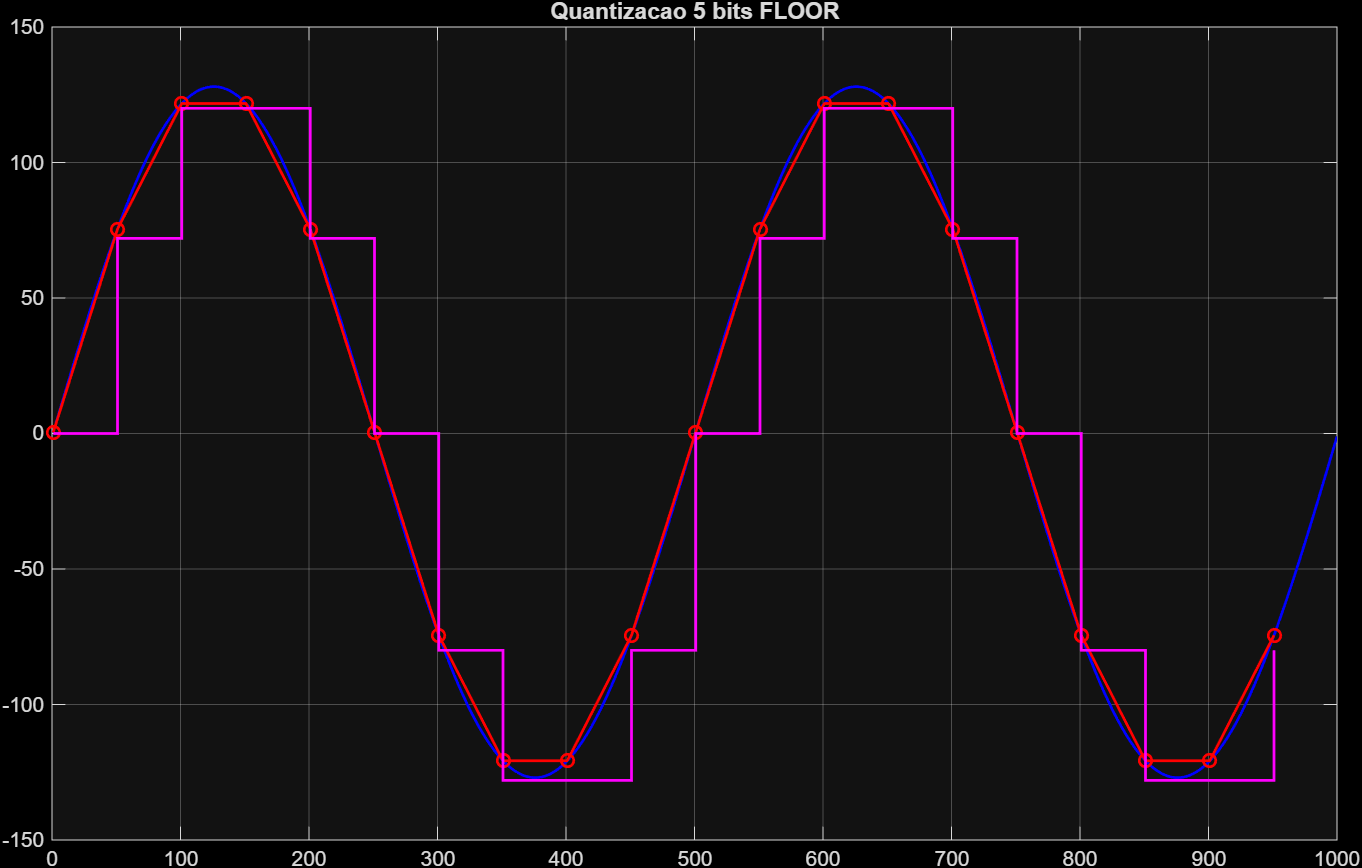
\includegraphics[width=0.85\textwidth]{imgs/q1d_floor_5bits.png}
    \caption{Quantização em 5 bits utilizando \texttt{floor}.}
\end{figure}

\begin{figure}[H]
    \centering
    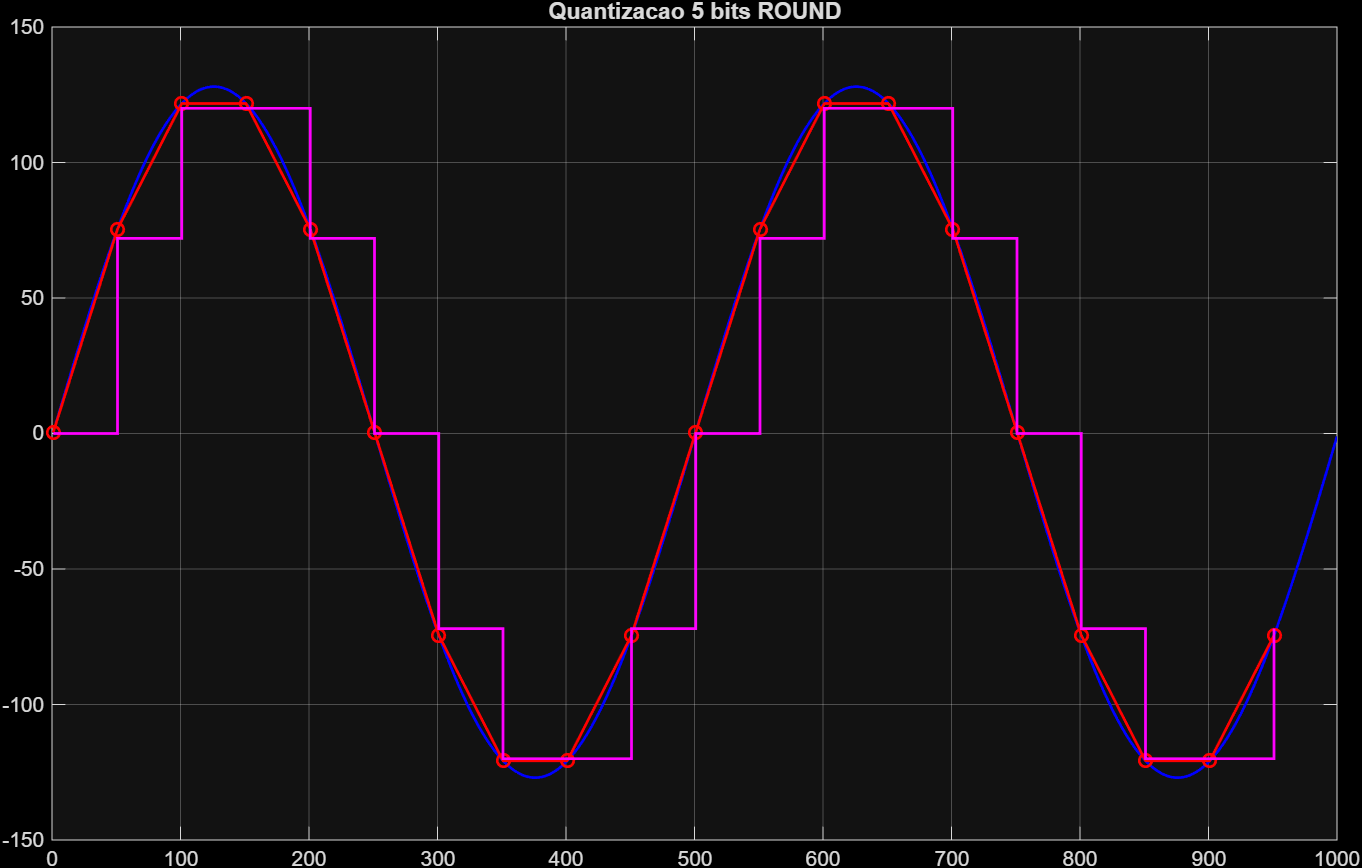
\includegraphics[width=0.85\textwidth]{imgs/q1d_round_5bits.png}
    \caption{Quantização em 5 bits utilizando \texttt{round}.}
\end{figure}

\textbf{Comparação 2 vs 5 bits:} A passagem de 4 para 32 níveis aumenta substancialmente a fidelidade da curva quantizada — o degrau acompanha de perto a senoide amostrada, formando uma escada bem mais densa onde antes havia apenas blocos largos. Cada bit adicional divide o erro máximo de quantização por dois; ao adicionar 3 bits ($\Delta M = 3$), o erro máximo se reduz em $2^{3}=8$ vezes (de $\pm 32$ para $\pm 4$ usando \texttt{round}). A relação sinal-ruído de quantização (SQNR) cresce a cada bit em aproximadamente $6{,}02$\,dB, o que significa que a transição de 2 para 5 bits melhora a SQNR em $\approx 18$\,dB — um ganho equivalente a multiplicar a potência do sinal útil por 64 em relação ao ruído de quantização. Em 5 bits o efeito do método de arredondamento (\texttt{floor} vs \texttt{round}) torna-se quase imperceptível visualmente, mas continua existindo: o \texttt{round} preserva a média do sinal (\textit{bias} nulo) enquanto o \texttt{floor} adiciona um \textit{offset} sistemático de $-\Delta/2 = -4$. Esse comportamento ilustra um princípio importante de projeto: aumentar o número de bits sempre ajuda na fidelidade, mas a escolha do método de arredondamento pode anular ou reforçar erros sistemáticos independentemente da resolução escolhida.

\clearpage
\section{Análise da taxa de amostragem mudando a frequência de amostragem}

\textbf{Enunciado:} ``Tomando 1 janela de 1\,s de um sinal senoidal ($V_P = 100$, $V_N = -100$), de frequência de 10\,Hz, varie a frequência de amostragem $f_s \in \{5,\,15,\,20,\,20{,}01,\,25,\,40\}$\,Hz. Para cada sinal obtido, calcule \texttt{abs(fft(sinal))}. Plot os sinais no tempo e na frequência em gráficos diferentes. Aqui a frequência do sinal é sempre 10\,Hz, o que muda é a frequência de amostragem. Tire suas conclusões para cada frequência, quanto a quando existe a recuperação do sinal ou quando ocorre o aliasing.''

\textbf{Exemplo de código fornecido (caso $f_s = 15$\,Hz):}
\begin{lstlisting}
figure(4);
s10original = senoide(100, -100, 10, 200); % sinal "continuo" 200 pontos
s10amostrado = senoide(100, -100, 10, 15); % amostrado com 15 amostras
indice = 1:200/15:200; % vetor de indice (15 amostras)
plot(s10original); hold on;
plot(indice, s10amostrado); % estica s10amostrado sobre s10original
hold off;
\end{lstlisting}

Cada caso é apresentado a seguir em duas figuras separadas: a primeira mostra o sinal amostrado (vermelho, com marcadores) sobreposto à versão ``contínua'' de 200 pontos (azul); a segunda mostra o módulo da FFT do sinal amostrado, com o eixo $k$ limitado de modo a destacar a região relevante do espectro discreto (até a metade do espectro de cada FFT).

\subsection{Caso $f_s = 5$\,Hz}

\begin{figure}[H]
    \centering
    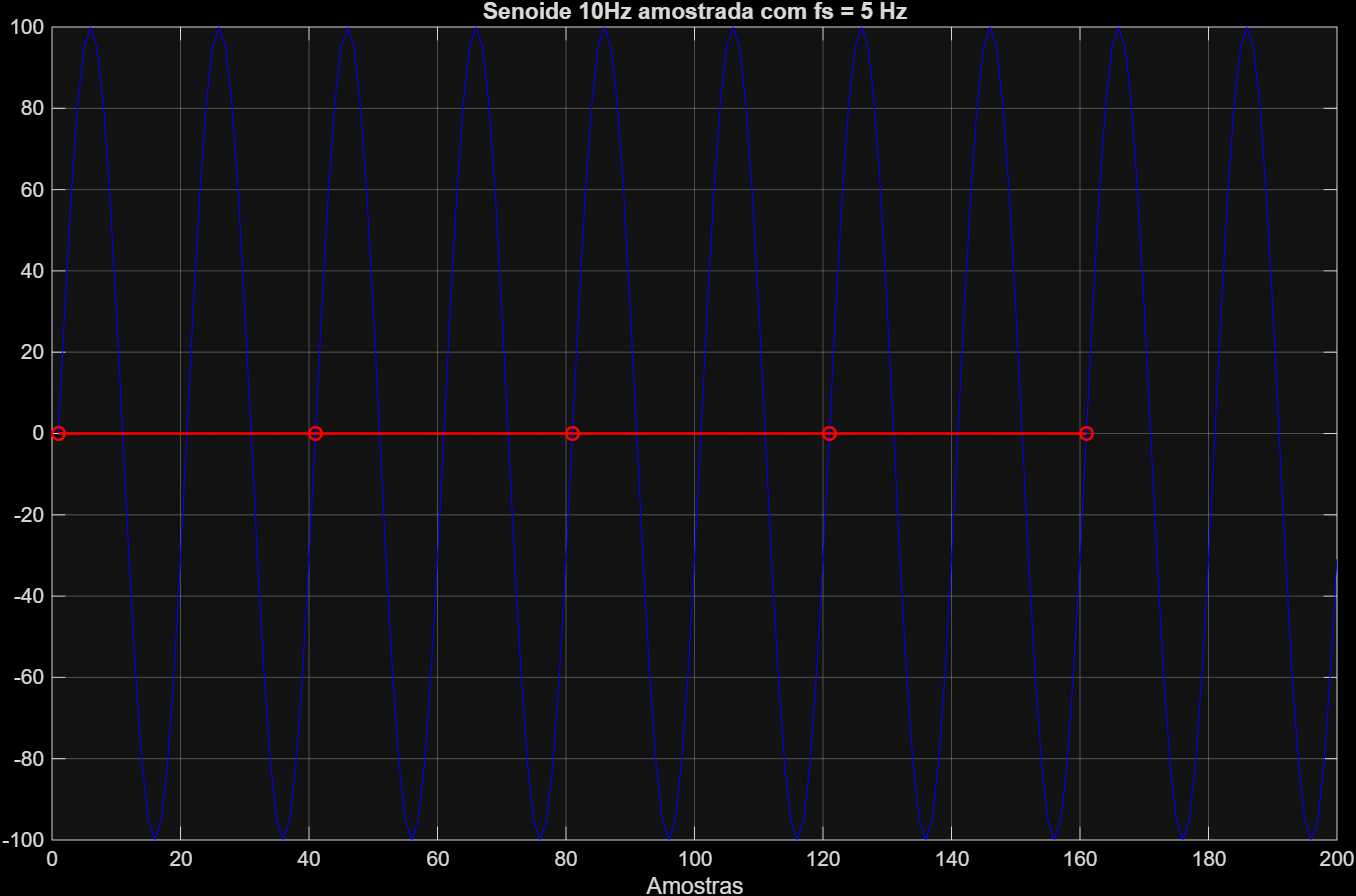
\includegraphics[width=0.85\textwidth]{imgs/q2_seno_5_tempo.png}
    \caption{Senoide 10\,Hz amostrada a $f_s = 5$\,Hz - representação no tempo.}
\end{figure}

\begin{figure}[H]
    \centering
    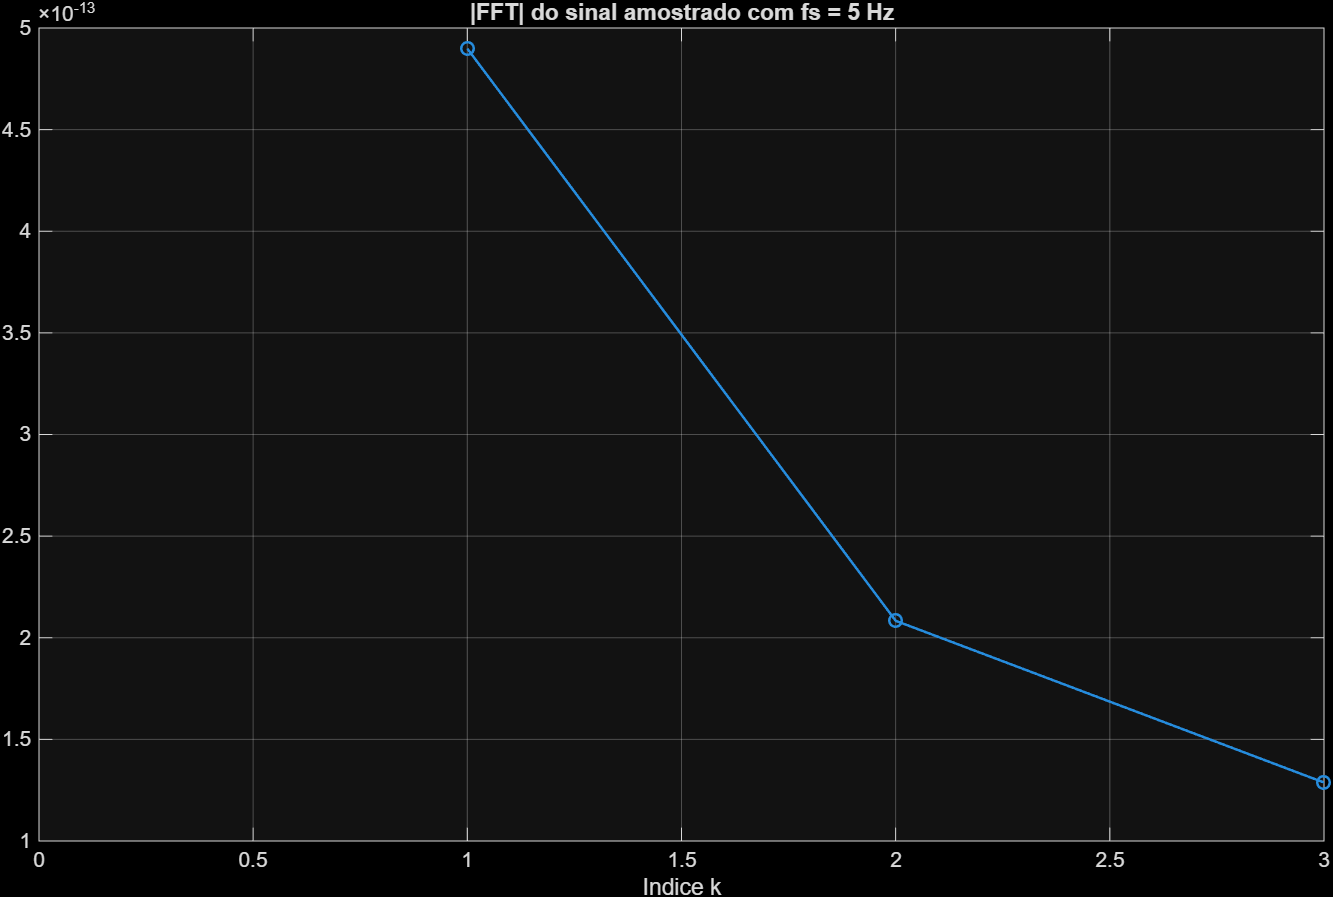
\includegraphics[width=0.85\textwidth]{imgs/q2_seno_5_fft.png}
    \caption{Senoide 10\,Hz amostrada a $f_s = 5$\,Hz - $|\text{FFT}|$ até $k=3$.}
\end{figure}

\subsection{Caso $f_s = 15$\,Hz}

\begin{figure}[H]
    \centering
    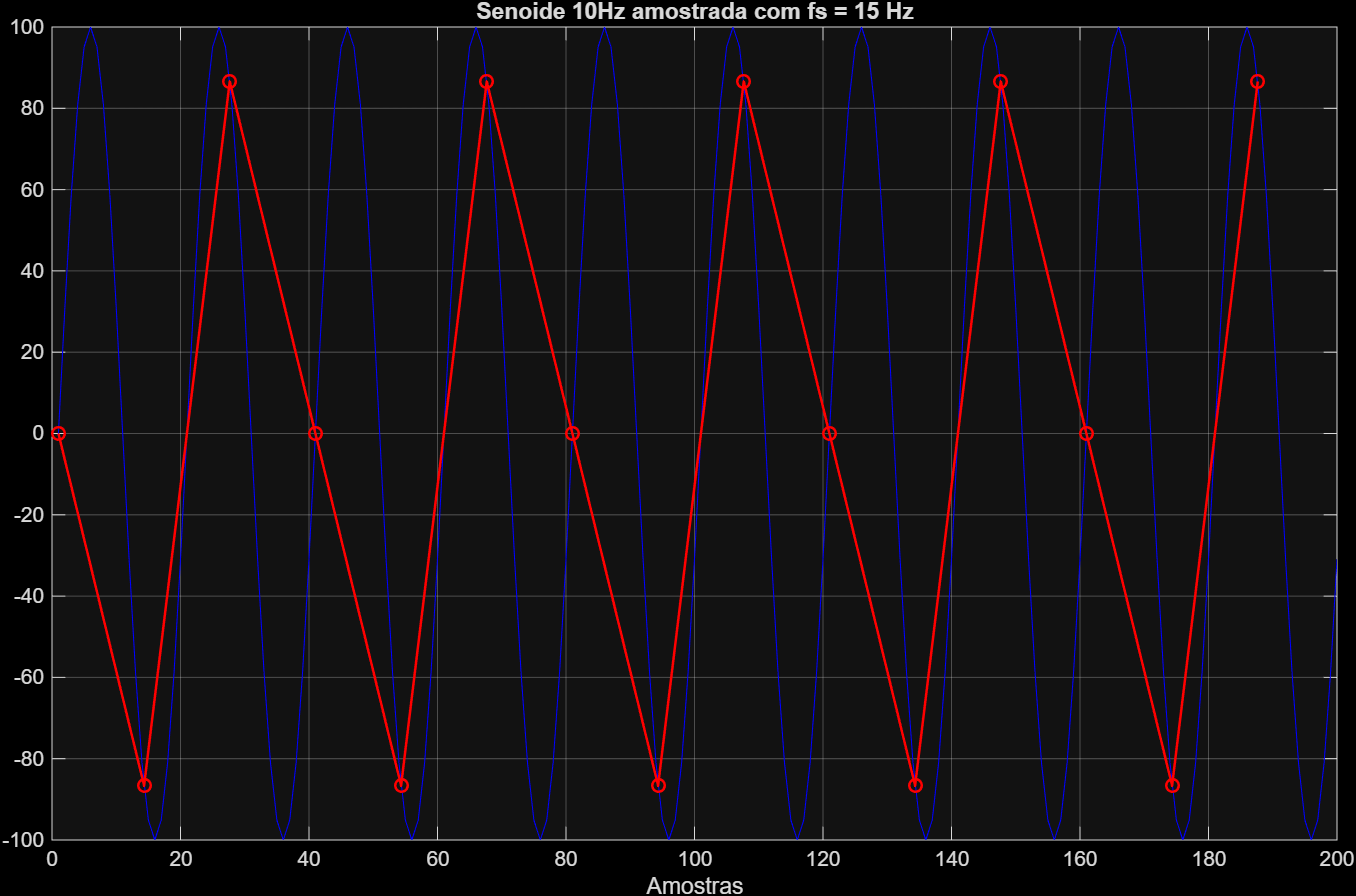
\includegraphics[width=0.85\textwidth]{imgs/q2_seno_15_tempo.png}
    \caption{Senoide 10\,Hz amostrada a $f_s = 15$\,Hz - representação no tempo.}
\end{figure}

\begin{figure}[H]
    \centering
    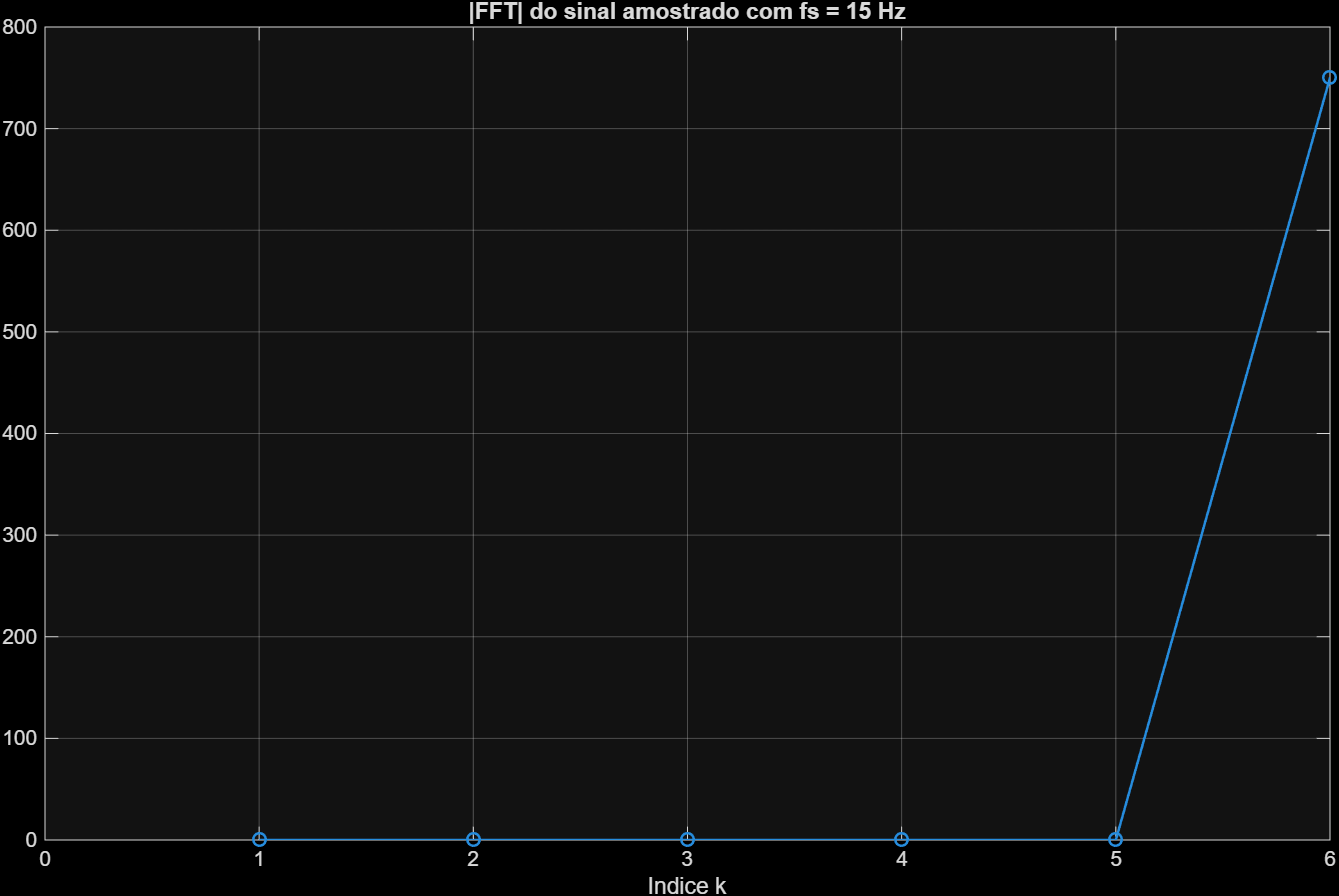
\includegraphics[width=0.85\textwidth]{imgs/q2_seno_15_fft.png}
    \caption{Senoide 10\,Hz amostrada a $f_s = 15$\,Hz - $|\text{FFT}|$ até $k=6$.}
\end{figure}

\subsection{Caso $f_s = 20$\,Hz}

\begin{figure}[H]
    \centering
    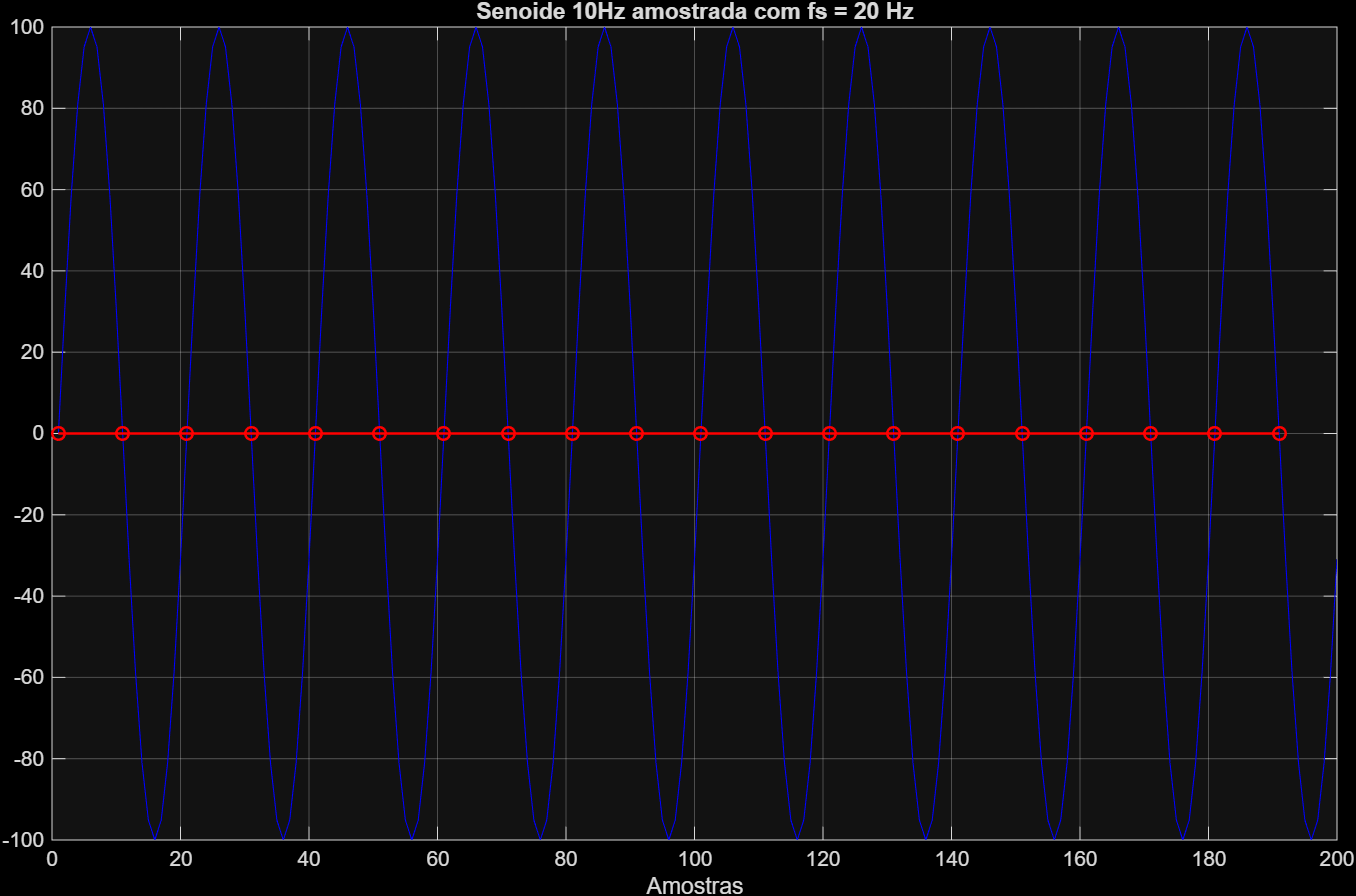
\includegraphics[width=0.85\textwidth]{imgs/q2_seno_20_tempo.png}
    \caption{Senoide 10\,Hz amostrada a $f_s = 20$\,Hz (caso limite de Nyquist) - representação no tempo.}
\end{figure}

\begin{figure}[H]
    \centering
    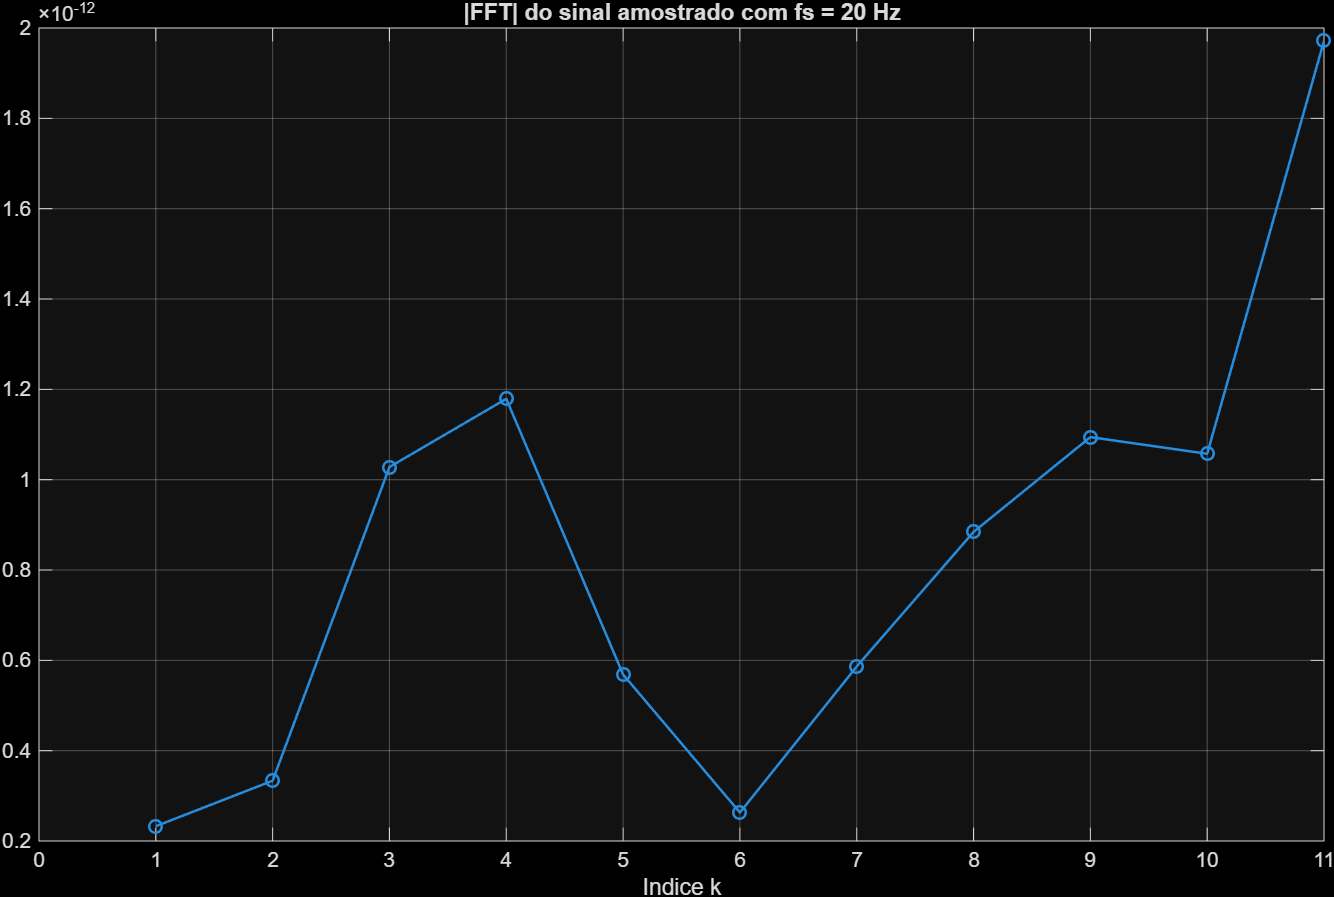
\includegraphics[width=0.85\textwidth]{imgs/q2_seno_20_fft.png}
    \caption{Senoide 10\,Hz amostrada a $f_s = 20$\,Hz - $|\text{FFT}|$ até $k=11$.}
\end{figure}

\subsection{Caso $f_s = 20{,}01$\,Hz}

\begin{figure}[H]
    \centering
    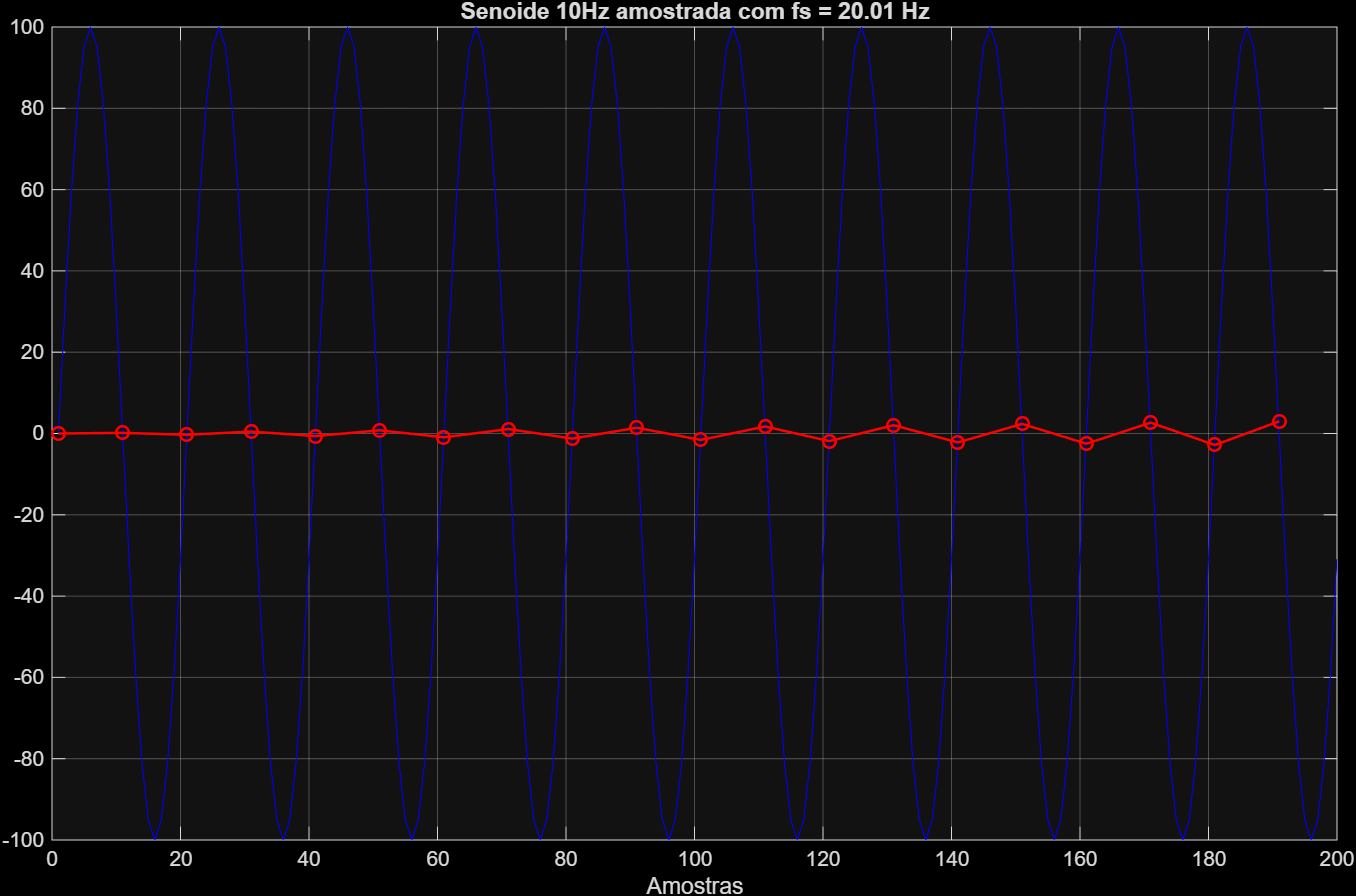
\includegraphics[width=0.85\textwidth]{imgs/q2_seno_20p01_tempo.png}
    \caption{Senoide 10\,Hz amostrada a $f_s = 20{,}01$\,Hz - representação no tempo.}
\end{figure}

\begin{figure}[H]
    \centering
    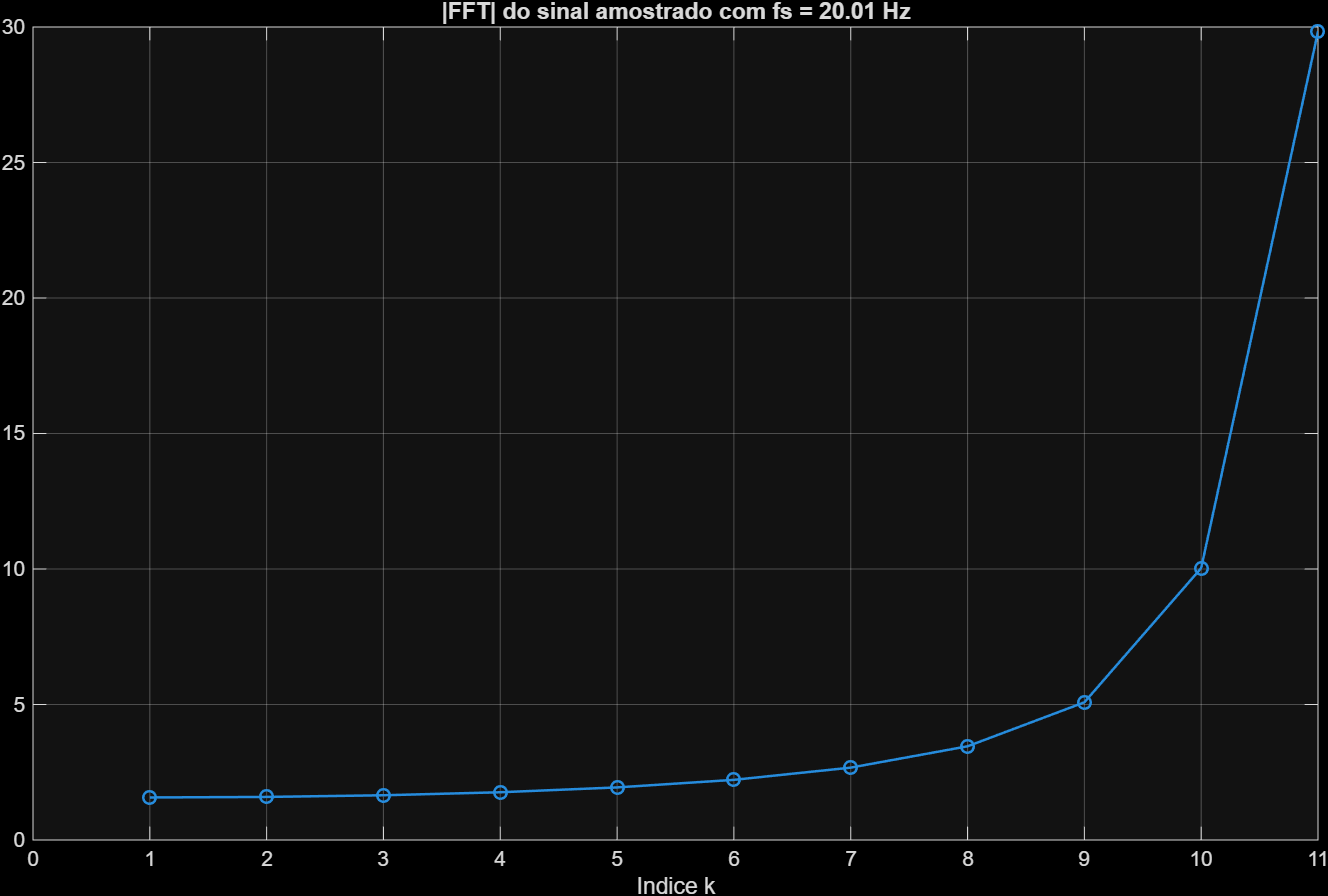
\includegraphics[width=0.85\textwidth]{imgs/q2_seno_20p01_fft.png}
    \caption{Senoide 10\,Hz amostrada a $f_s = 20{,}01$\,Hz - $|\text{FFT}|$ até $k=11$.}
\end{figure}

\subsection{Caso $f_s = 25$\,Hz}

\begin{figure}[H]
    \centering
    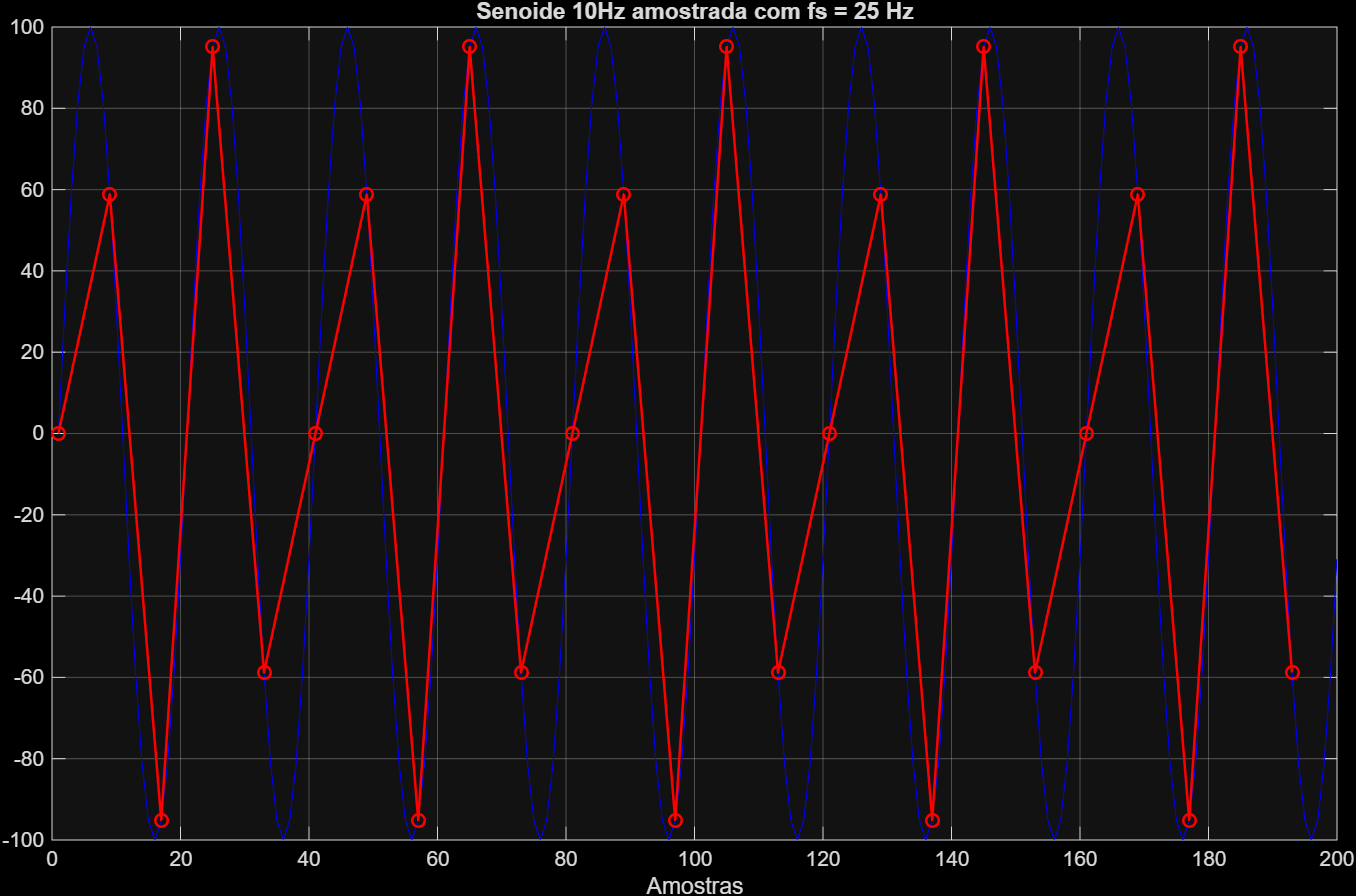
\includegraphics[width=0.85\textwidth]{imgs/q2_seno_25_tempo.png}
    \caption{Senoide 10\,Hz amostrada a $f_s = 25$\,Hz - representação no tempo.}
\end{figure}

\begin{figure}[H]
    \centering
    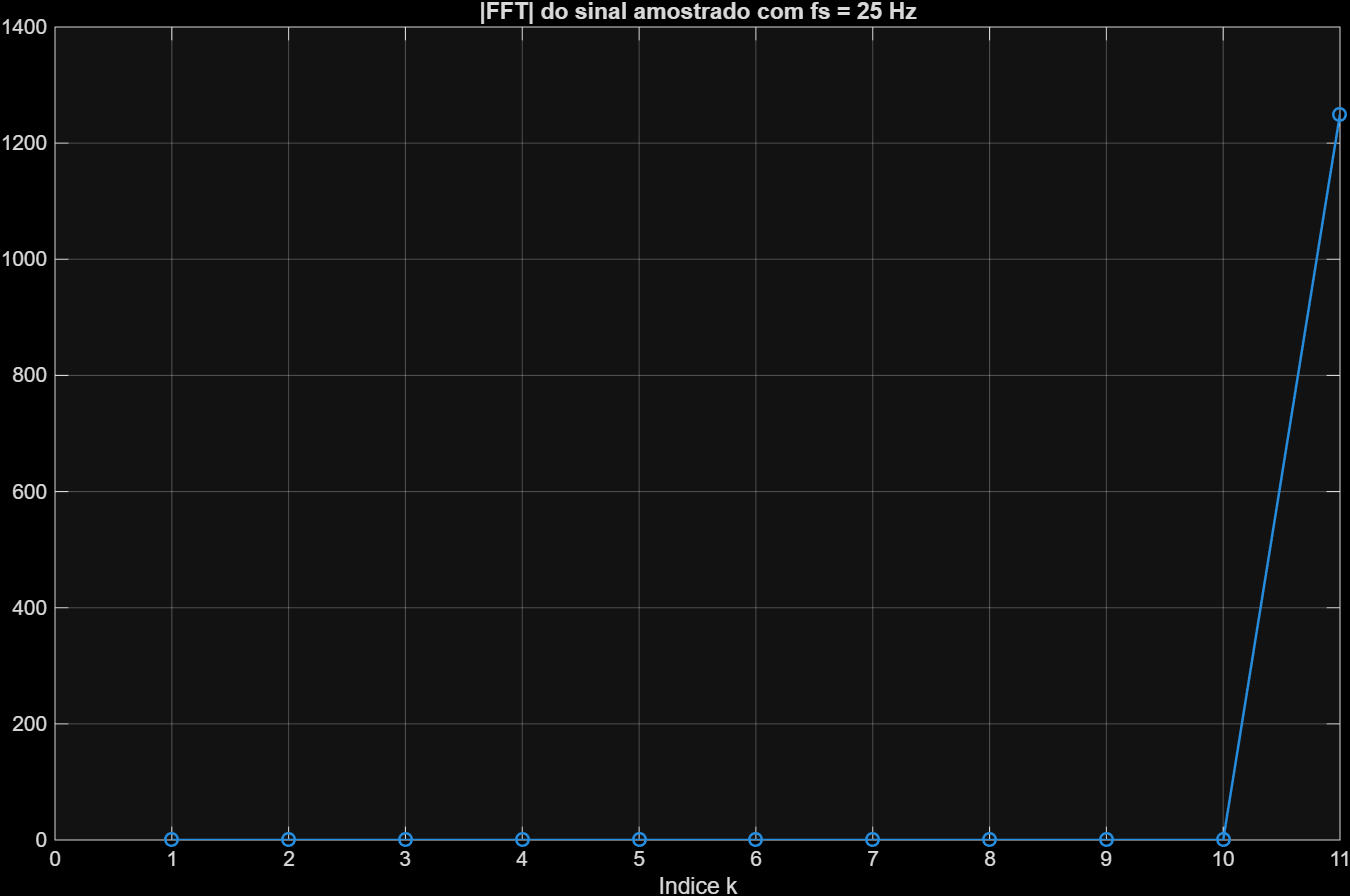
\includegraphics[width=0.85\textwidth]{imgs/q2_seno_25_fft.png}
    \caption{Senoide 10\,Hz amostrada a $f_s = 25$\,Hz - $|\text{FFT}|$ até $k=11$.}
\end{figure}

\subsection{Caso $f_s = 40$\,Hz}

\begin{figure}[H]
    \centering
    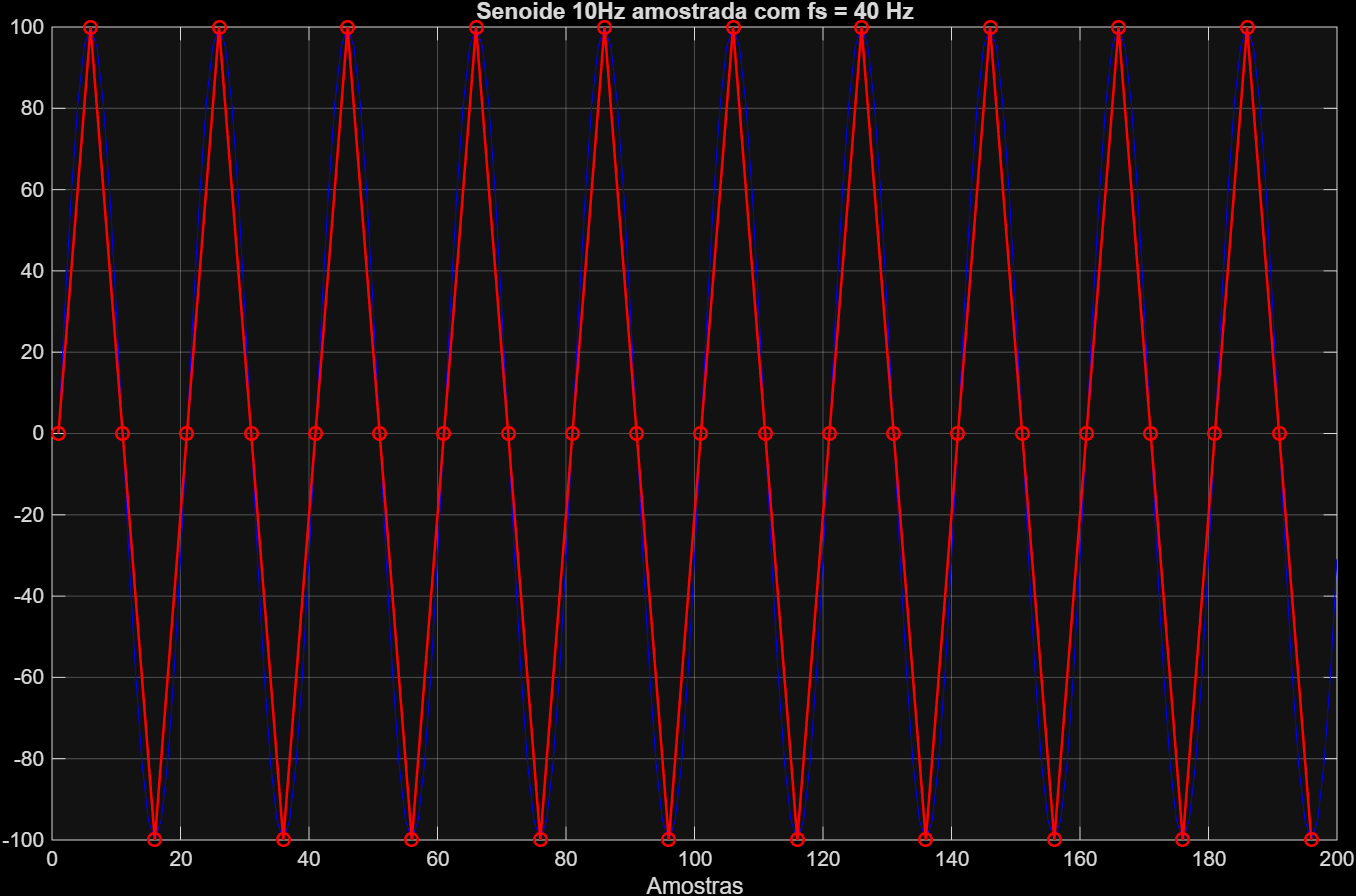
\includegraphics[width=0.85\textwidth]{imgs/q2_seno_40_tempo.png}
    \caption{Senoide 10\,Hz amostrada a $f_s = 40$\,Hz - representação no tempo.}
\end{figure}

\begin{figure}[H]
    \centering
    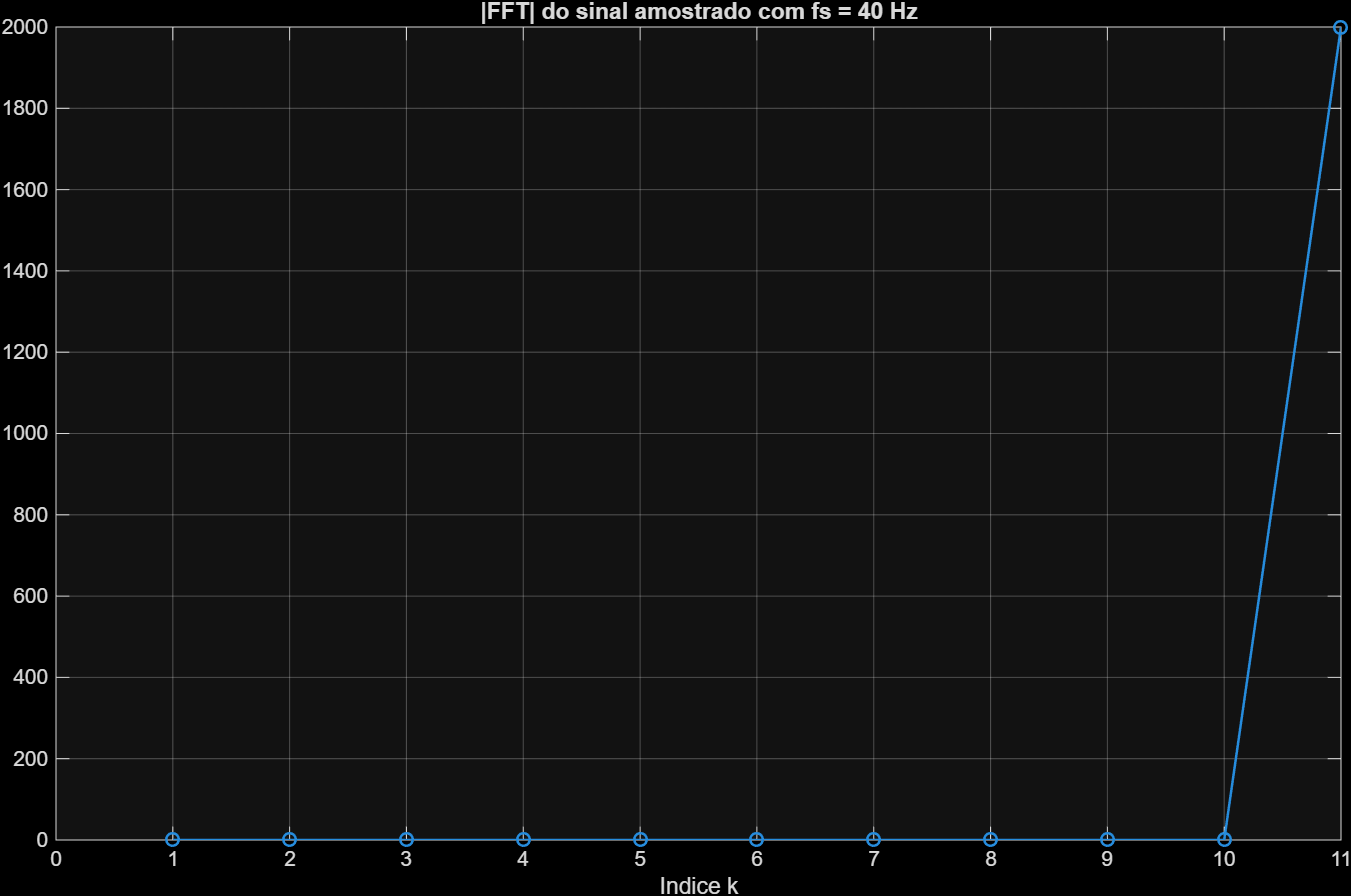
\includegraphics[width=0.85\textwidth]{imgs/q2_seno_40_fft.png}
    \caption{Senoide 10\,Hz amostrada a $f_s = 40$\,Hz - $|\text{FFT}|$ até $k=11$.}
\end{figure}

\subsection{Observação sobre $f_s = 20{,}01$\,Hz com 4000 amostras}

\textbf{Enunciado:} ``OBS: Antes de explicar o que acontece com a frequência de amostragem de 20,01\,Hz, faça:''

\begin{lstlisting}
for i = 1:4000
    x(i) = 100*sin(2*pi*10*i/20.01); % apenas para 20,01 Hz
end
plot(x, 'o-')
\end{lstlisting}

\begin{figure}[H]
    \centering
    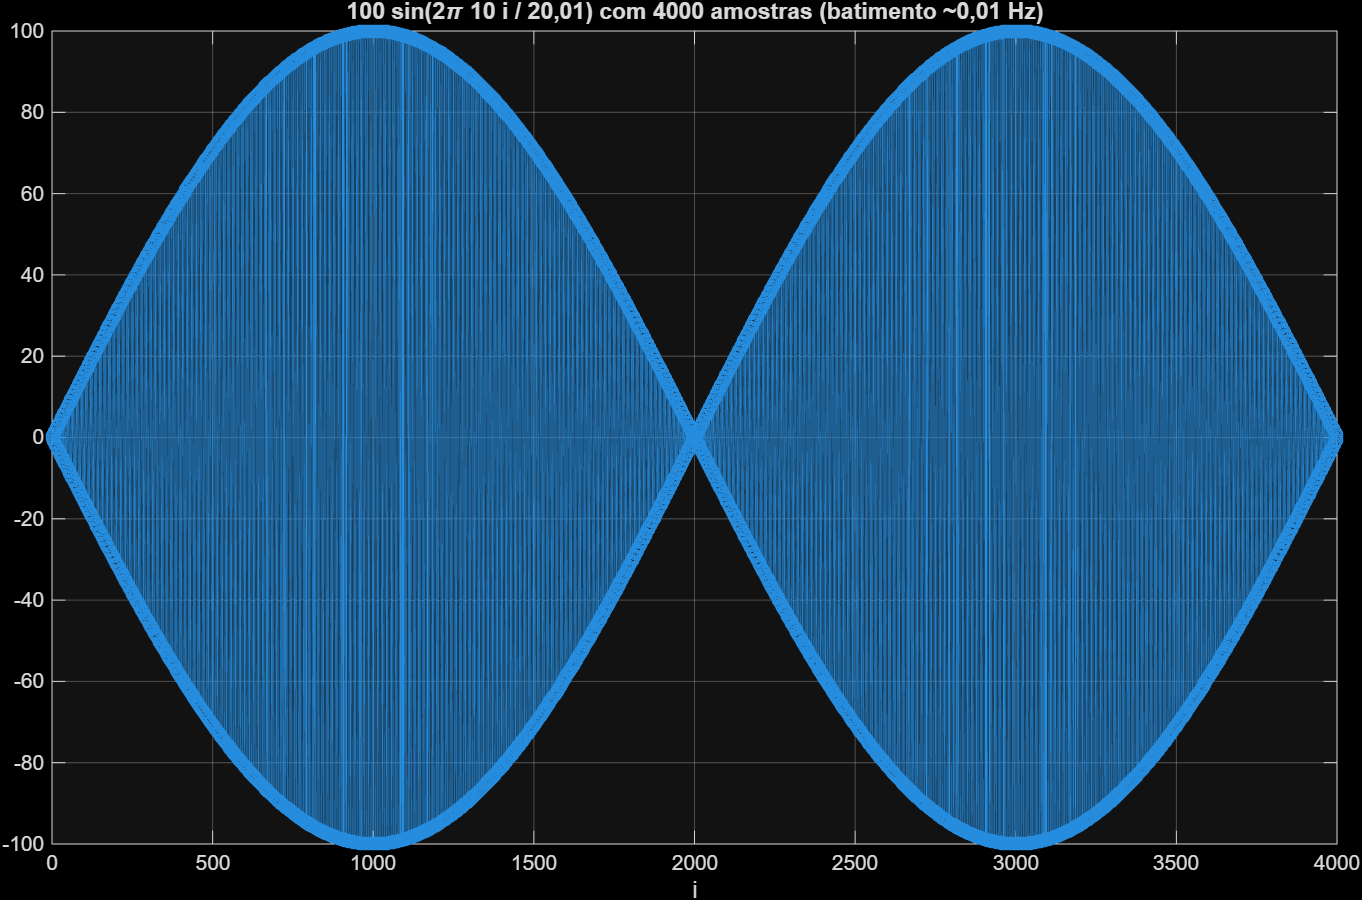
\includegraphics[width=0.85\textwidth]{imgs/q2_batimento_2001.png}
    \caption{$100\sin(2\pi\cdot 10\cdot i/20{,}01)$ com 4000 amostras: aparece um envelope de batimento de aproximadamente $\Delta f = 20{,}01-2\cdot 10 = 0{,}01$\,Hz.}
\end{figure}

\textbf{Interpretação:} A amostragem em $f_s = 20{,}01$\,Hz fica imediatamente acima do limite de Nyquist ($2f = 20$\,Hz), com folga de apenas $0{,}01$\,Hz. Cada amostra ``escorrega'' uma fração mínima do período, fazendo com que a fase do seno reconstruído gire muito lentamente em relação à fase verdadeira. O resultado é um \emph{batimento}: o sinal amostrado parece amplitude-modulado por uma envoltória de frequência $\Delta f = f_s - 2f = 0{,}01$\,Hz (período de 100\,s, equivalente a $\sim 2000$ amostras na taxa $f_s$). Esse fenômeno demonstra que mesmo \emph{cumprindo} o critério de Nyquist por uma margem muito pequena, a reconstrução em janelas curtas pode falhar visualmente, e na prática deve-se trabalhar com $f_s \geq 2{,}5\,f$ ou superior para garantir robustez.

\subsection{Conclusões item a item — recuperação ou aliasing}

\begin{itemize}
    \item \textbf{$f_s = 5$\,Hz}: $f_s/2 = 2{,}5$\,Hz $<$ 10\,Hz. Critério de Nyquist gravemente violado: a frequência de amostragem está \emph{abaixo} da do próprio sinal, então cada período de 0{,}1\,s do sinal é representado por apenas meia amostra. Ocorre aliasing severo — todas as amostras caem em zeros do seno (pois $10/5 = 2$ é inteiro), resultando em valores numericamente nulos. A FFT (limitada a $k \in [0,3]$) mostra apenas ruído de ponto flutuante (ordem de $10^{-13}$) e a forma temporal é uma reta horizontal de zeros.

    \item \textbf{$f_s = 15$\,Hz}: $f_s/2 = 7{,}5$\,Hz $<$ 10\,Hz. Ainda há aliasing — o pico da FFT aparece deslocado, refletindo a frequência \textit{aparente} $|f - f_s| = |10-15| = 5$\,Hz. Em uma FFT de 15 pontos com taxa $f_s=15$\,Hz, a raia de 5\,Hz cai em $k = 5\cdot 15/15 + 1 = 6$ (e seu espelho em $k=11$, fora da janela $k \in [0,6]$ mostrada). A senoide reconstruída no tempo aparenta ter período ${\sim}3$ amostras = $1/5$\,s, ou seja, um sinal aparente de 5\,Hz, totalmente distinto do sinal original.

    \item \textbf{$f_s = 20$\,Hz}: $f_s/2 = 10$\,Hz $=$ $f$. Caso limite de Nyquist. A teoria de Shannon garante recuperação somente em condições ideais (janela infinita e amostragem perfeitamente em fase). Na prática, a FFT (mostrada até $k=11$) apresenta um pico em $k=11$ correspondente exatamente à frequência $f = (k-1)\cdot f_s/N = 10\cdot 20/20 = 10$\,Hz, mas o sinal no tempo apresenta amplitudes irregulares — todos os zeros ou todos os picos podem ser amostrados, dependendo da fase relativa. Para senoide amostrada nos cruzamentos por zero, o sinal reconstruído é identicamente nulo.

    \item \textbf{$f_s = 20{,}01$\,Hz}: $f_s/2 = 10{,}005$\,Hz $>$ 10\,Hz. Existe recuperação no sentido estrito do teorema, porém a margem é tão pequena que se manifesta como o batimento de envelope $\sim 0{,}01$\,Hz já discutido. A FFT já apresenta pico bem definido em $k=11$ correspondente a $\approx 10$\,Hz, mostrando que o conteúdo espectral está ali, mas a janela curta de 20 amostras não captura a oscilação do envelope, dando a impressão de amplitude irregular no tempo.

    \item \textbf{$f_s = 25$\,Hz}: $f_s/2 = 12{,}5$\,Hz $>$ 10\,Hz. Recuperação confortável; a margem de 2{,}5\,Hz acima do dobro da frequência do sinal é suficiente para uma reconstrução visualmente reconhecível. O pico da FFT em $k=11$ é nítido (correspondendo a $10\cdot 25/25=10$\,Hz) e a forma de onda já segue bem a senoide original, embora ainda com distorção visível por estar abaixo de $f_s = 4f$.

    \item \textbf{$f_s = 40$\,Hz}: $f_s/2 = 20$\,Hz $\gg$ 10\,Hz. Reconstrução praticamente perfeita; o sinal no tempo se sobrepõe à senoide contínua e a FFT tem o pico bem definido em $k=11$. Nessa relação ($f_s = 4f$), cada período do sinal é representado por 4 amostras, suficientes para uma visualização limpa da forma de onda. Esta é a região prática de operação para qualquer sistema que precise não só recuperar matematicamente o sinal, mas também exibi-lo ou processá-lo sem artefatos.
\end{itemize}

\clearpage
\section{Repita todo o item 2) agora com uma cossenoide de 10\,Hz}

Repetem-se os mesmos experimentos para uma cossenoide de mesma frequência (10\,Hz), $V_P=100$, $V_N=-100$ e janela de 1\,s.

\subsection{Caso $f_s = 5$\,Hz}

\begin{figure}[H]
    \centering
    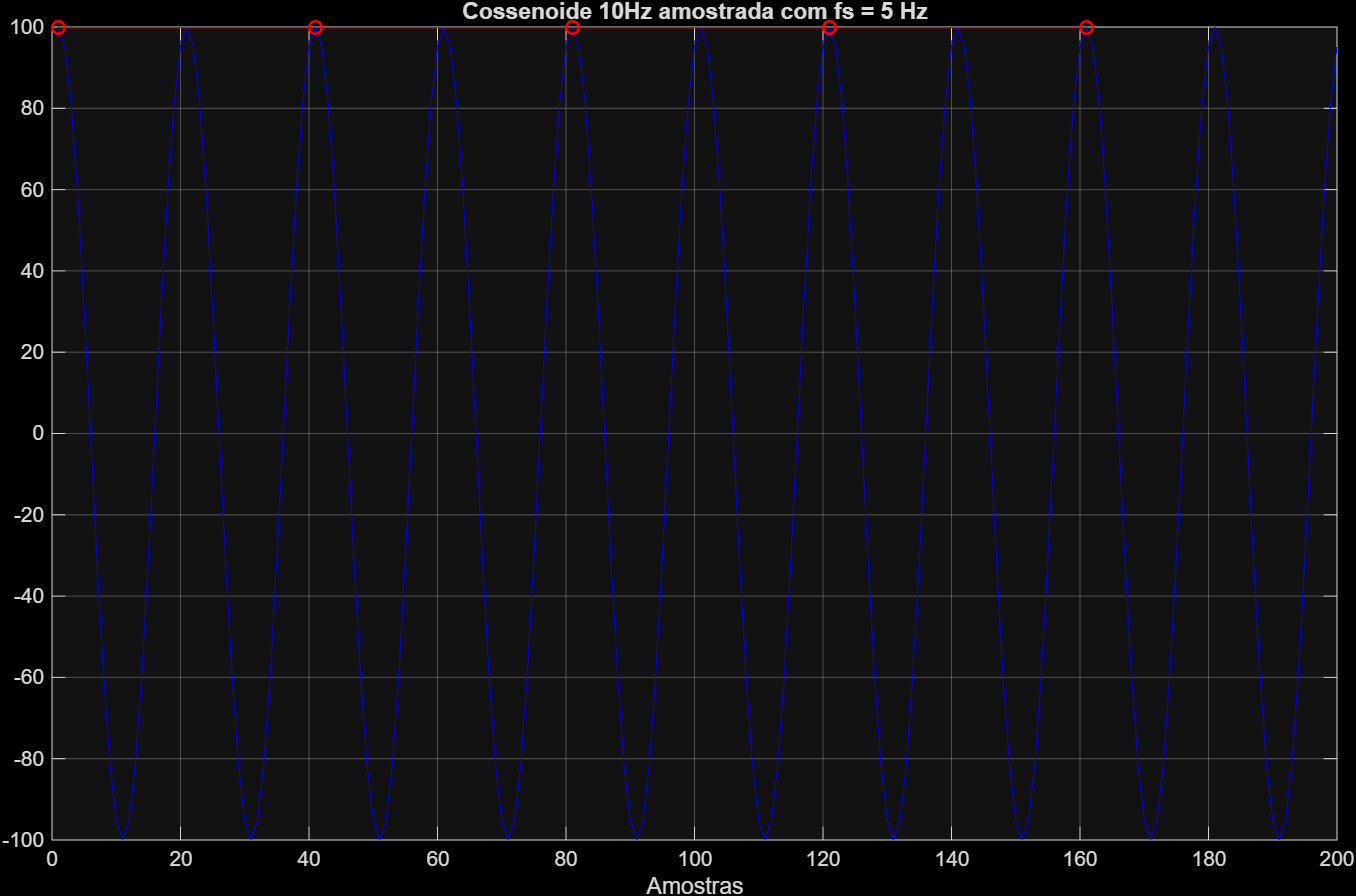
\includegraphics[width=0.85\textwidth]{imgs/q3_cos_5_tempo.png}
    \caption{Cossenoide 10\,Hz amostrada a $f_s = 5$\,Hz - representação no tempo.}
\end{figure}

\begin{figure}[H]
    \centering
    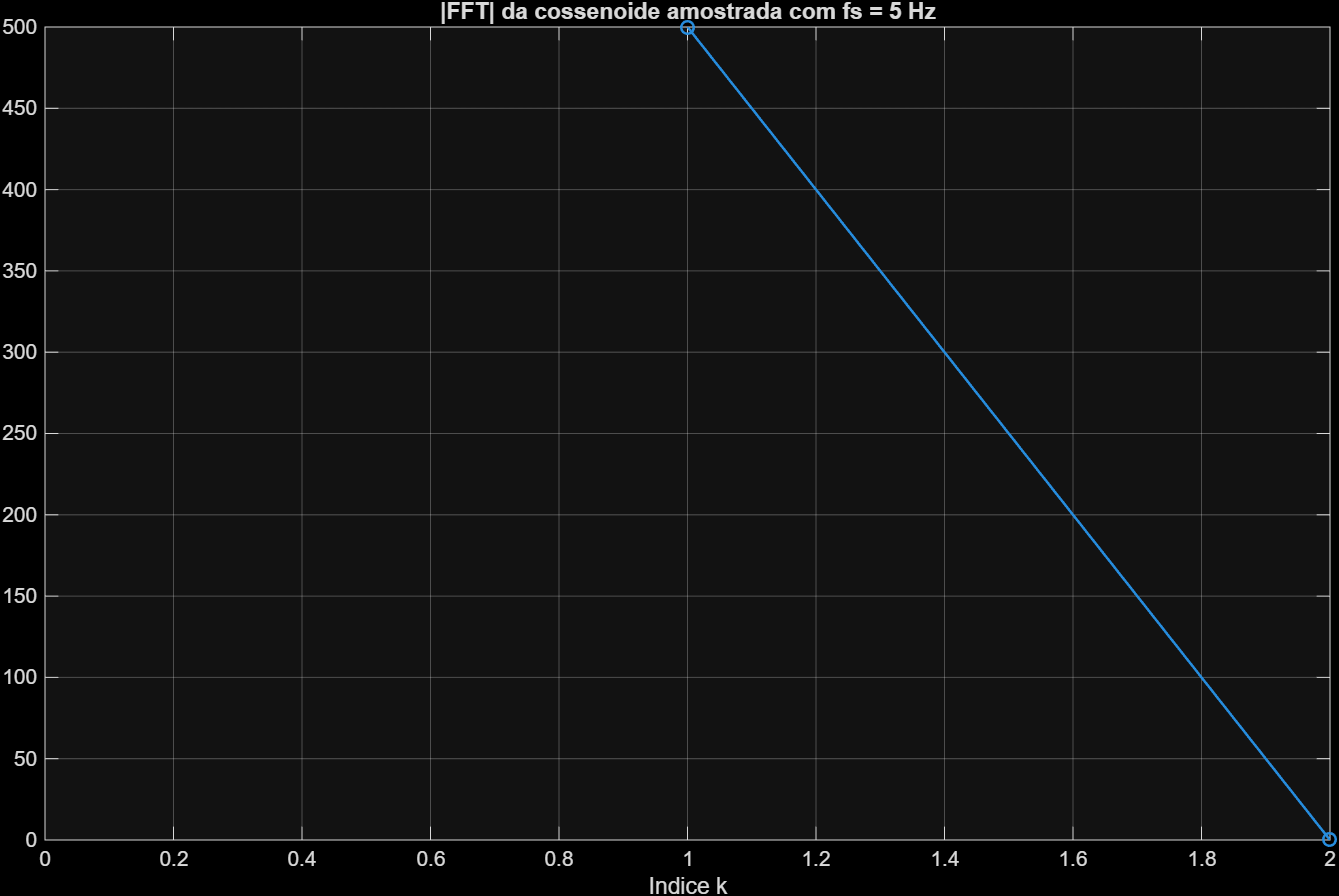
\includegraphics[width=0.85\textwidth]{imgs/q3_cos_5_fft.png}
    \caption{Cossenoide 10\,Hz amostrada a $f_s = 5$\,Hz - $|\text{FFT}|$ até $k=2$.}
\end{figure}

\subsection{Caso $f_s = 15$\,Hz}

\begin{figure}[H]
    \centering
    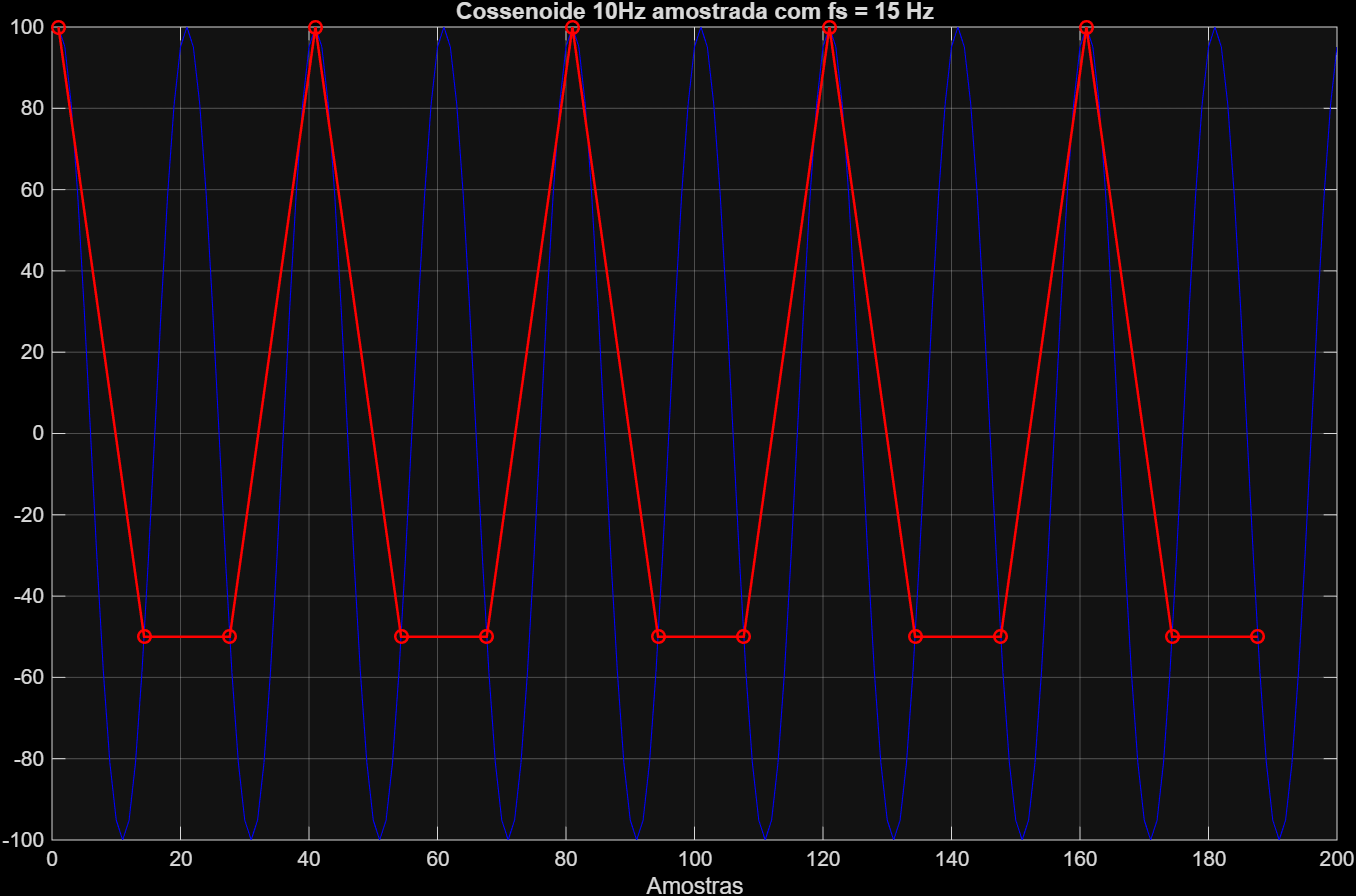
\includegraphics[width=0.85\textwidth]{imgs/q3_cos_15_tempo.png}
    \caption{Cossenoide 10\,Hz amostrada a $f_s = 15$\,Hz - representação no tempo.}
\end{figure}

\begin{figure}[H]
    \centering
    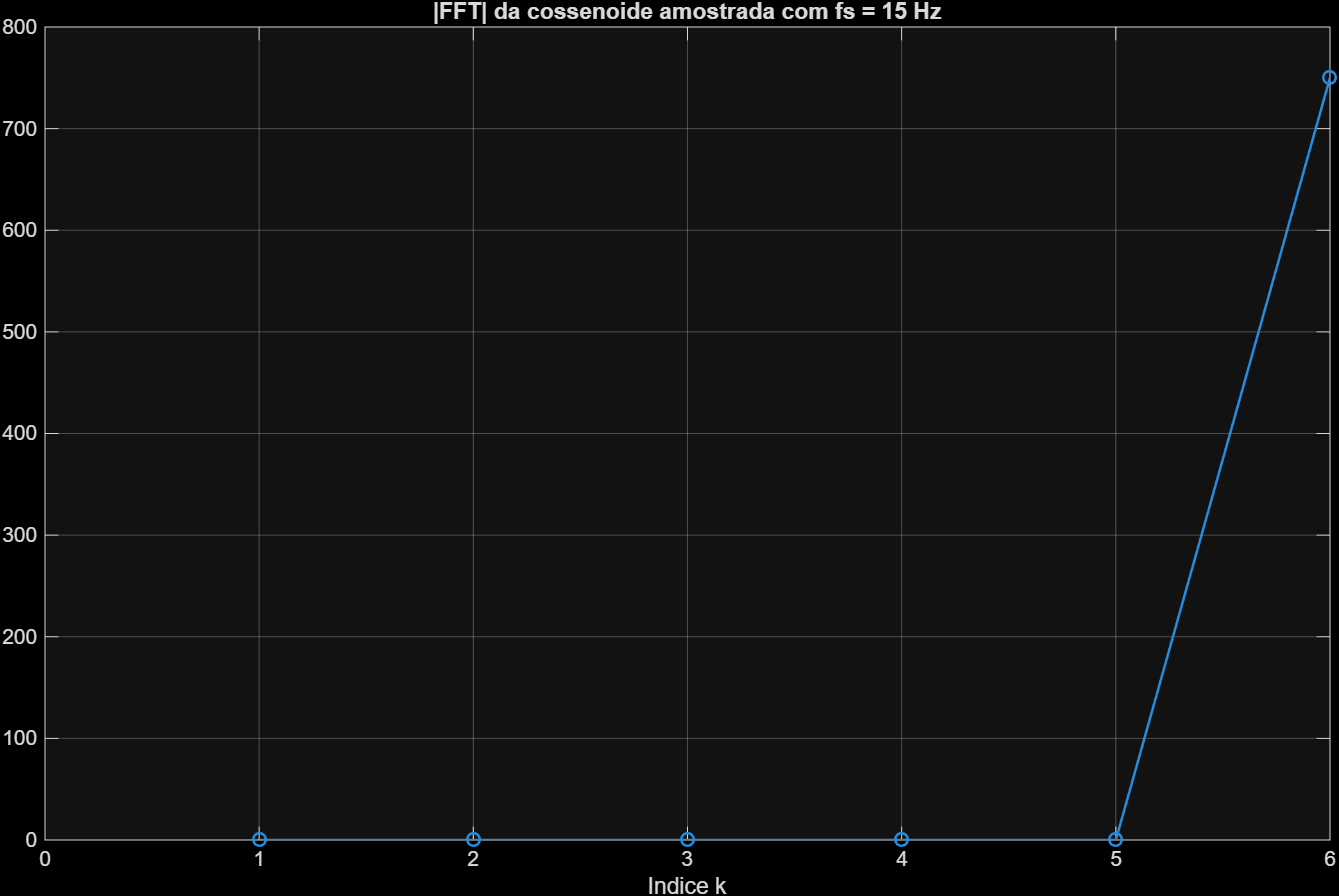
\includegraphics[width=0.85\textwidth]{imgs/q3_cos_15_fft.png}
    \caption{Cossenoide 10\,Hz amostrada a $f_s = 15$\,Hz - $|\text{FFT}|$ até $k=6$.}
\end{figure}

\subsection{Caso $f_s = 20$\,Hz}

\begin{figure}[H]
    \centering
    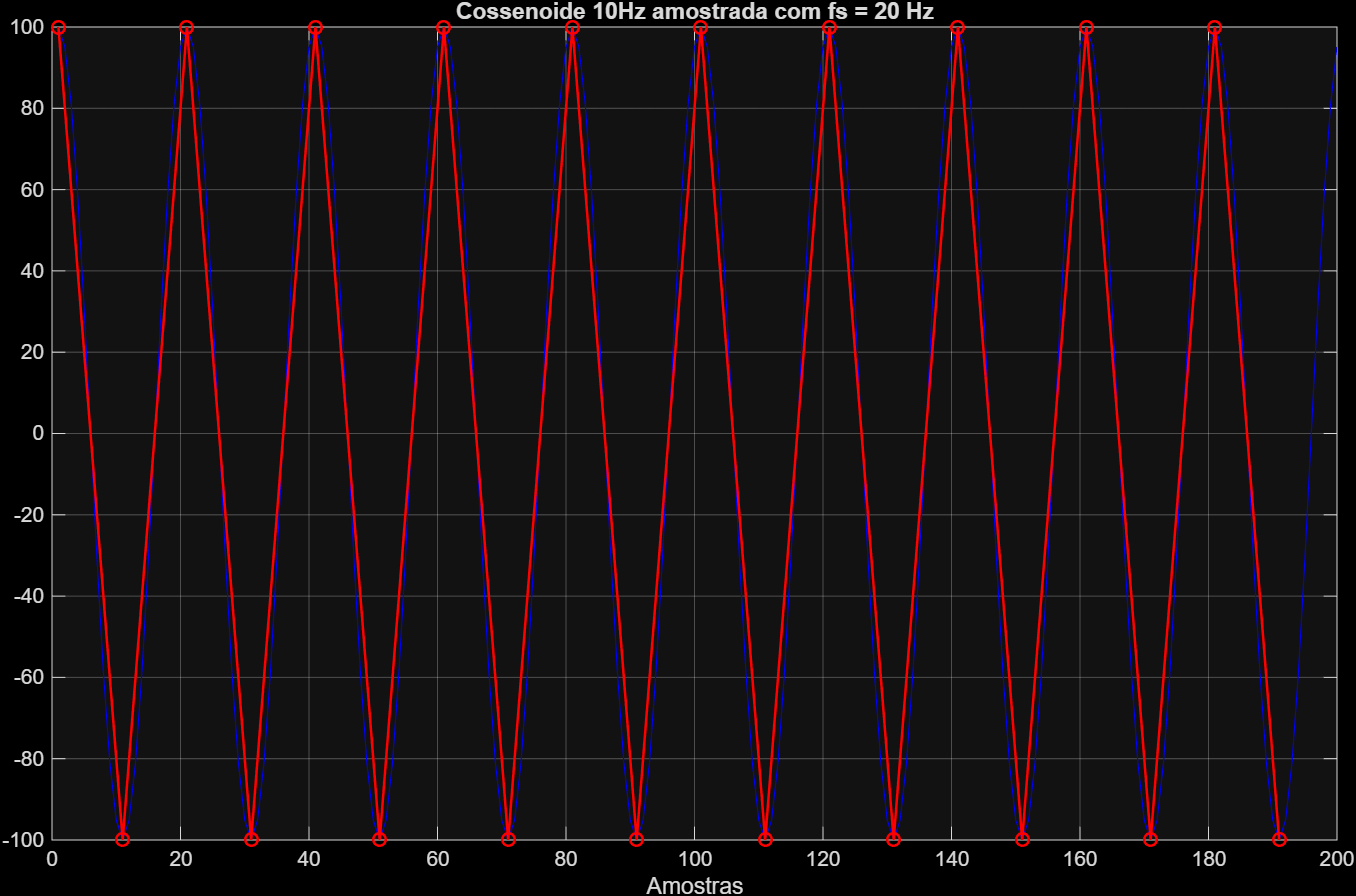
\includegraphics[width=0.85\textwidth]{imgs/q3_cos_20_tempo.png}
    \caption{Cossenoide 10\,Hz amostrada a $f_s = 20$\,Hz - representação no tempo.}
\end{figure}

\begin{figure}[H]
    \centering
    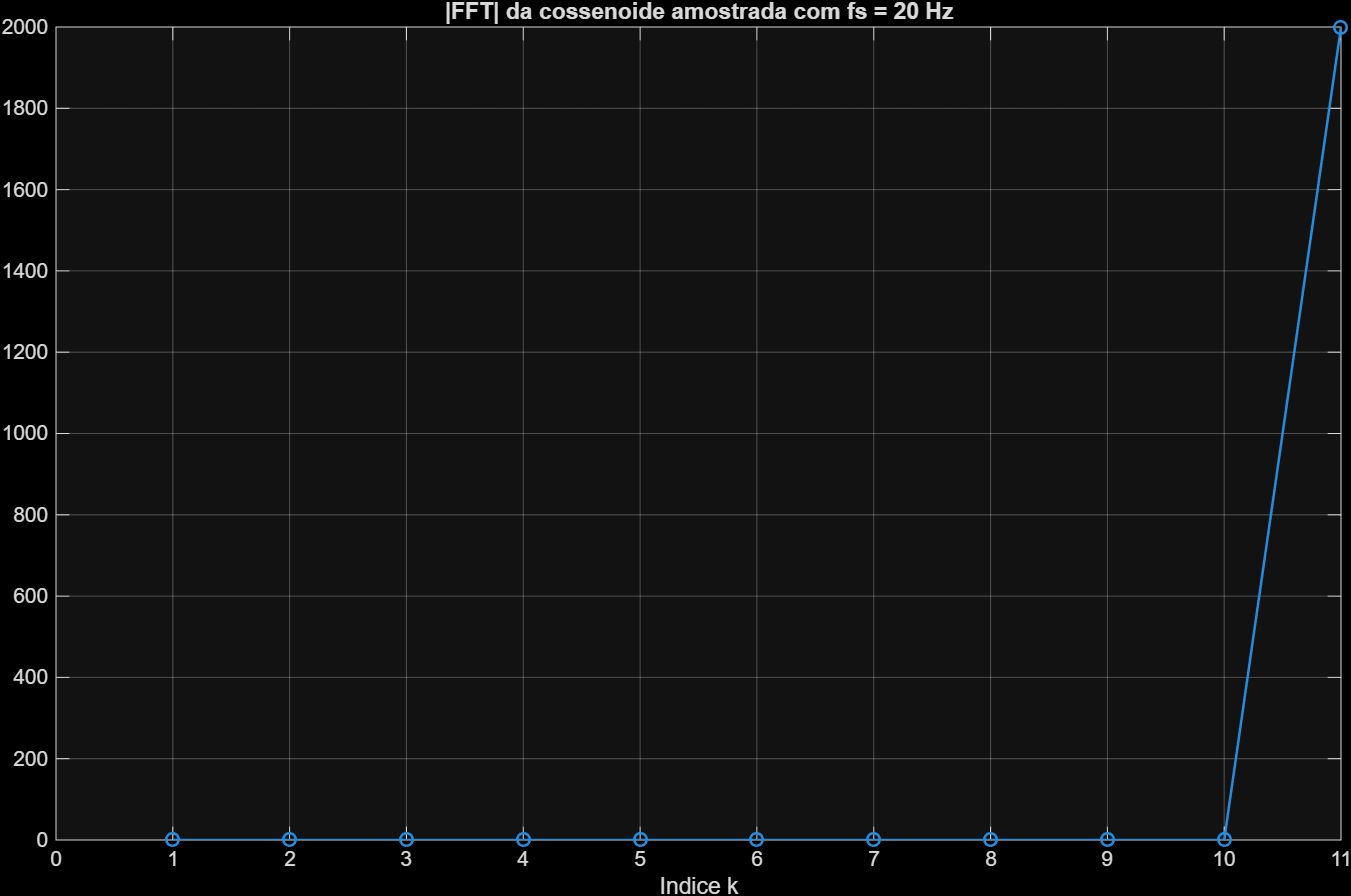
\includegraphics[width=0.85\textwidth]{imgs/q3_cos_20_fft.png}
    \caption{Cossenoide 10\,Hz amostrada a $f_s = 20$\,Hz - $|\text{FFT}|$ até $k=11$.}
\end{figure}

\subsection{Caso $f_s = 20{,}01$\,Hz}

\begin{figure}[H]
    \centering
    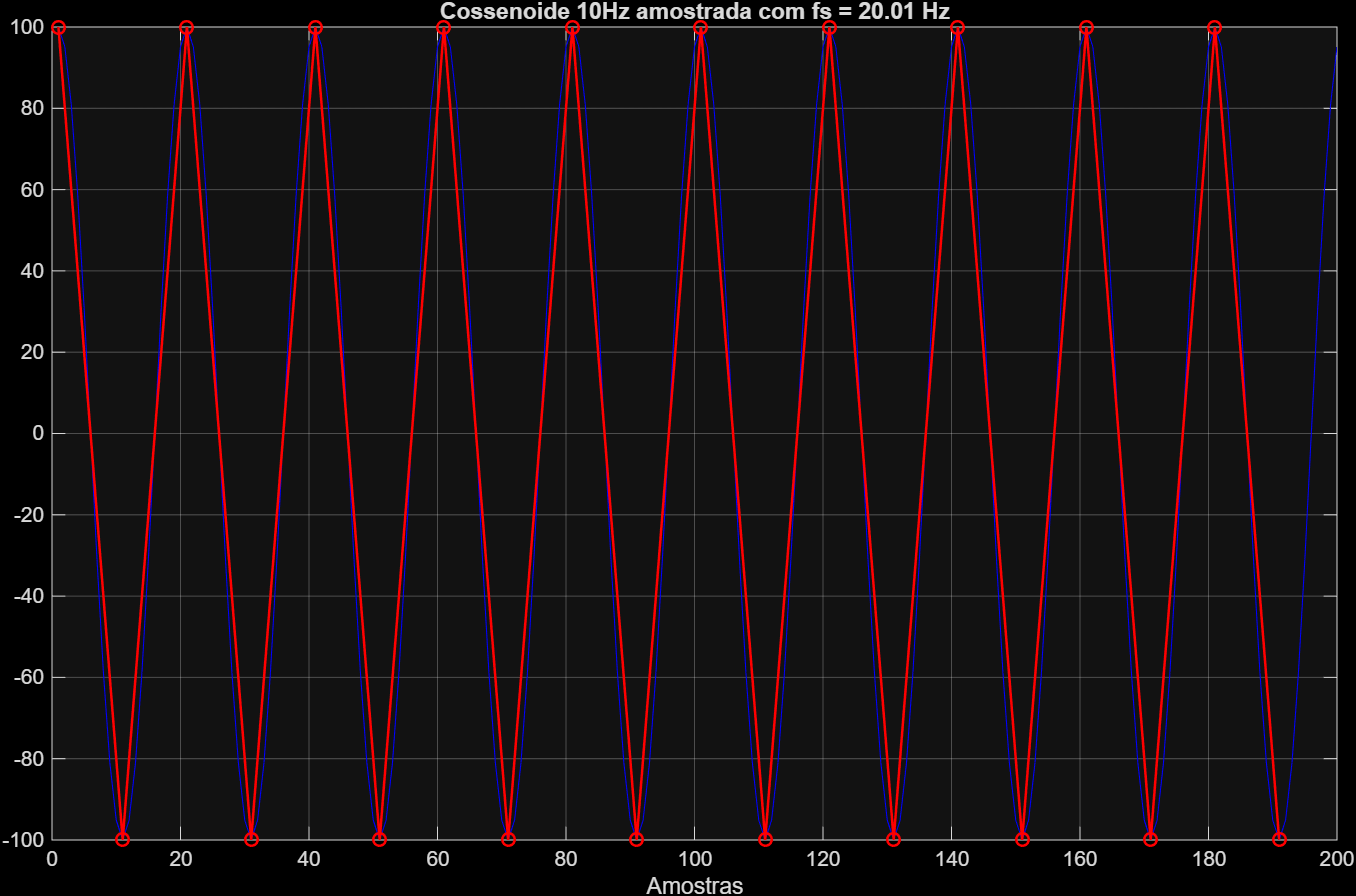
\includegraphics[width=0.85\textwidth]{imgs/q3_cos_20p01_tempo.png}
    \caption{Cossenoide 10\,Hz amostrada a $f_s = 20{,}01$\,Hz - representação no tempo.}
\end{figure}

\begin{figure}[H]
    \centering
    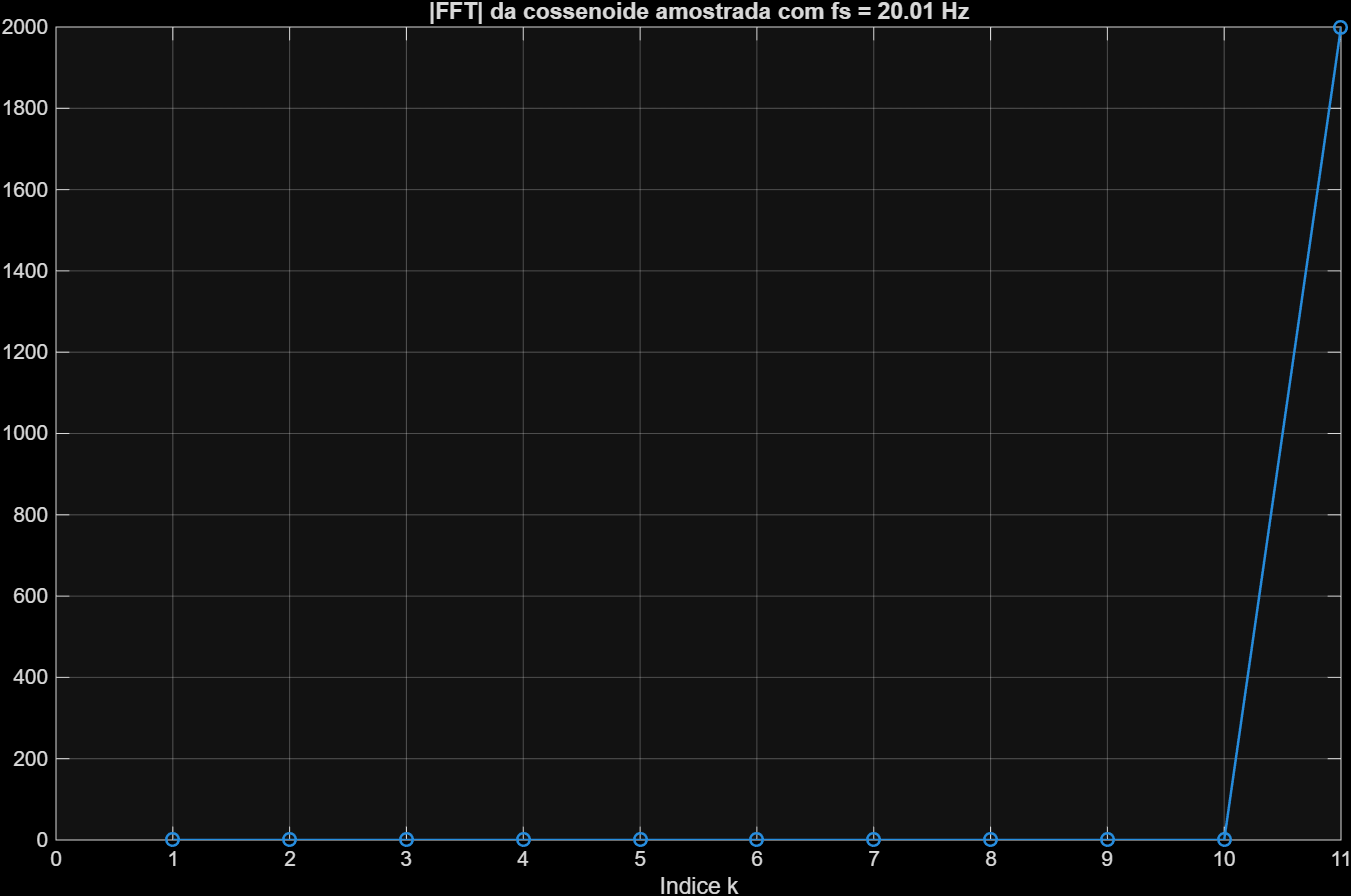
\includegraphics[width=0.85\textwidth]{imgs/q3_cos_20p01_fft.png}
    \caption{Cossenoide 10\,Hz amostrada a $f_s = 20{,}01$\,Hz - $|\text{FFT}|$ até $k=11$.}
\end{figure}

\subsection{Caso $f_s = 25$\,Hz}

\begin{figure}[H]
    \centering
    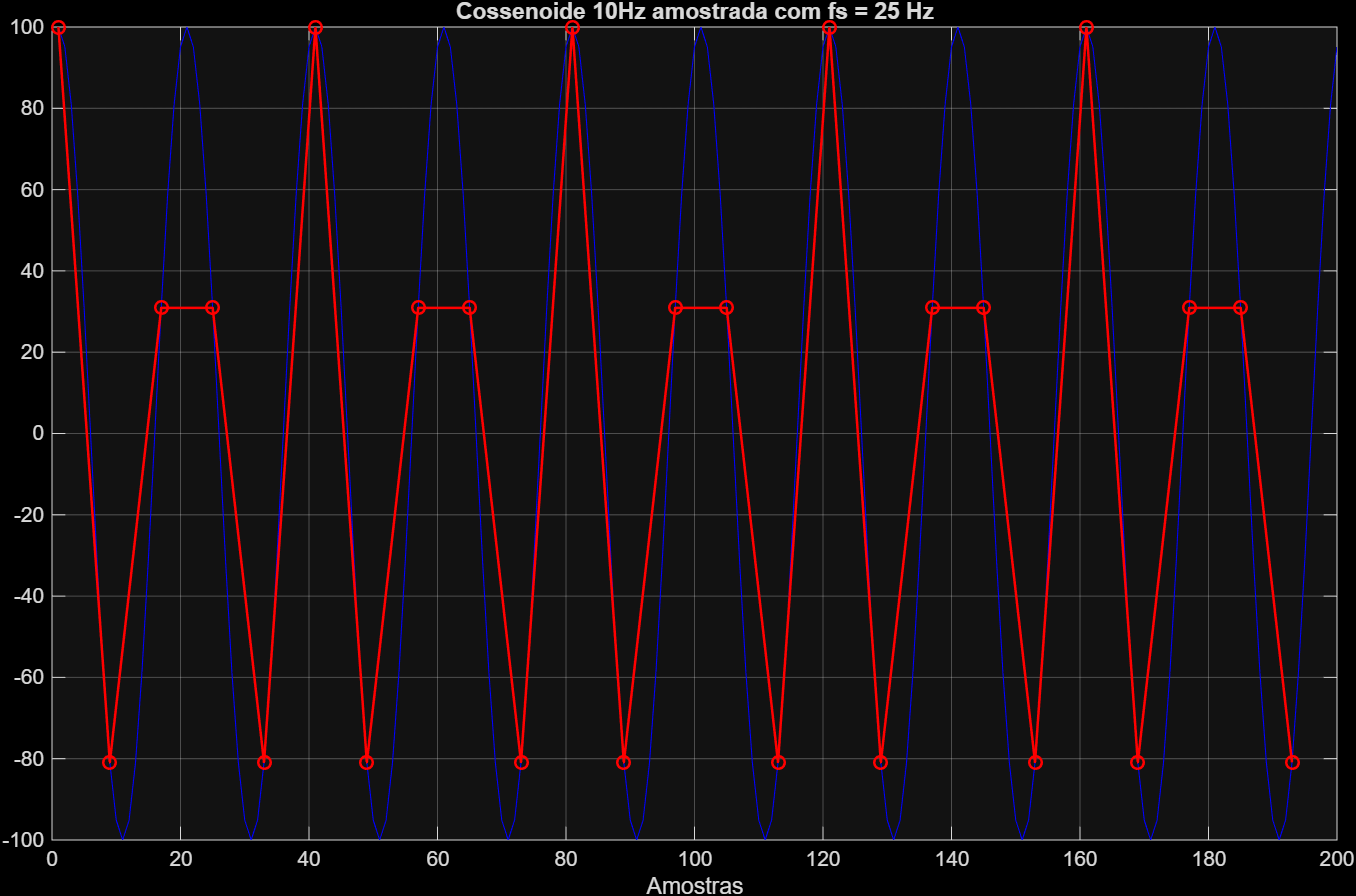
\includegraphics[width=0.85\textwidth]{imgs/q3_cos_25_tempo.png}
    \caption{Cossenoide 10\,Hz amostrada a $f_s = 25$\,Hz - representação no tempo.}
\end{figure}

\begin{figure}[H]
    \centering
    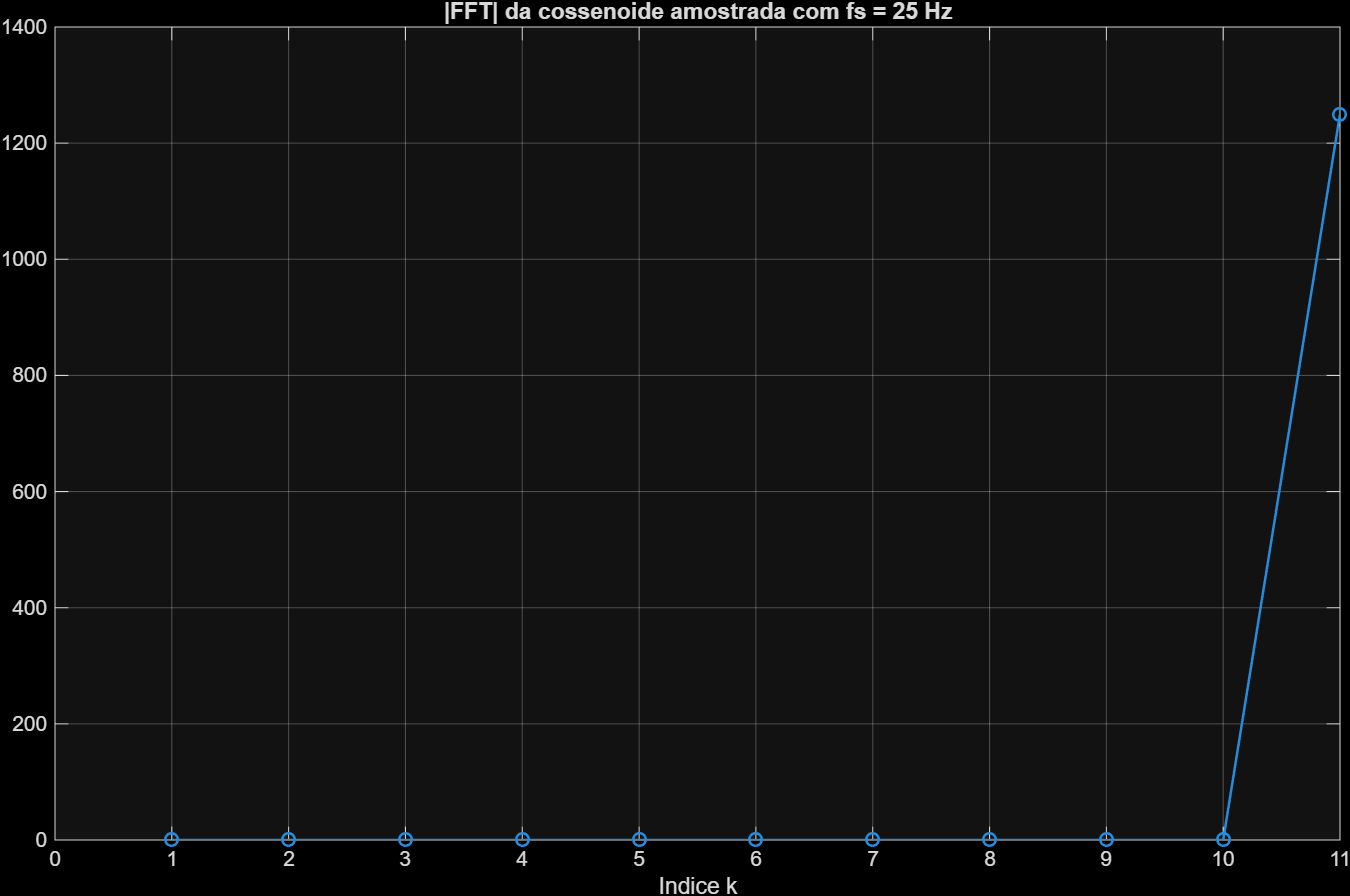
\includegraphics[width=0.85\textwidth]{imgs/q3_cos_25_fft.png}
    \caption{Cossenoide 10\,Hz amostrada a $f_s = 25$\,Hz - $|\text{FFT}|$ até $k=11$.}
\end{figure}

\subsection{Caso $f_s = 40$\,Hz}

\begin{figure}[H]
    \centering
    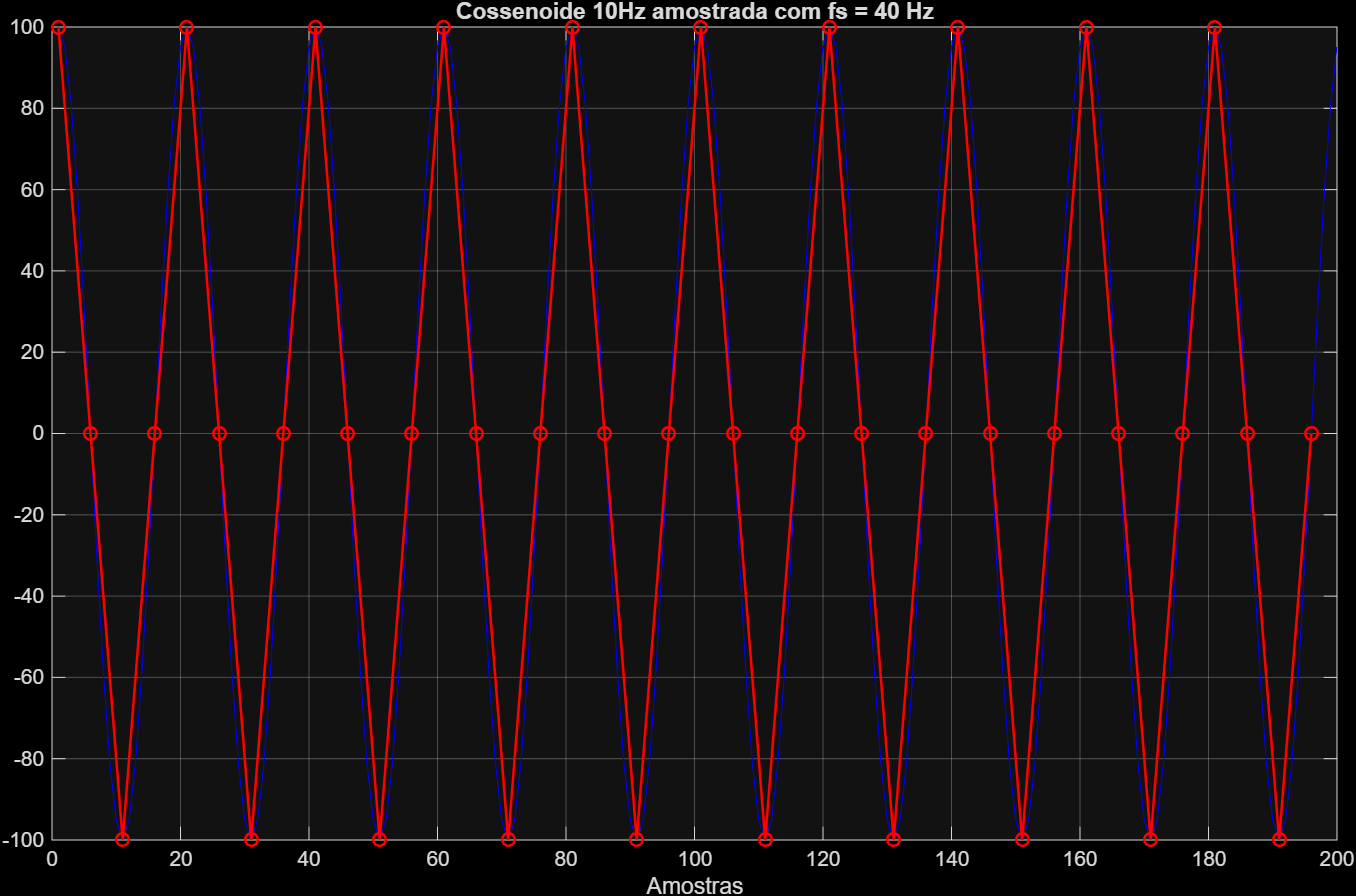
\includegraphics[width=0.85\textwidth]{imgs/q3_cos_40_tempo.png}
    \caption{Cossenoide 10\,Hz amostrada a $f_s = 40$\,Hz - representação no tempo.}
\end{figure}

\begin{figure}[H]
    \centering
    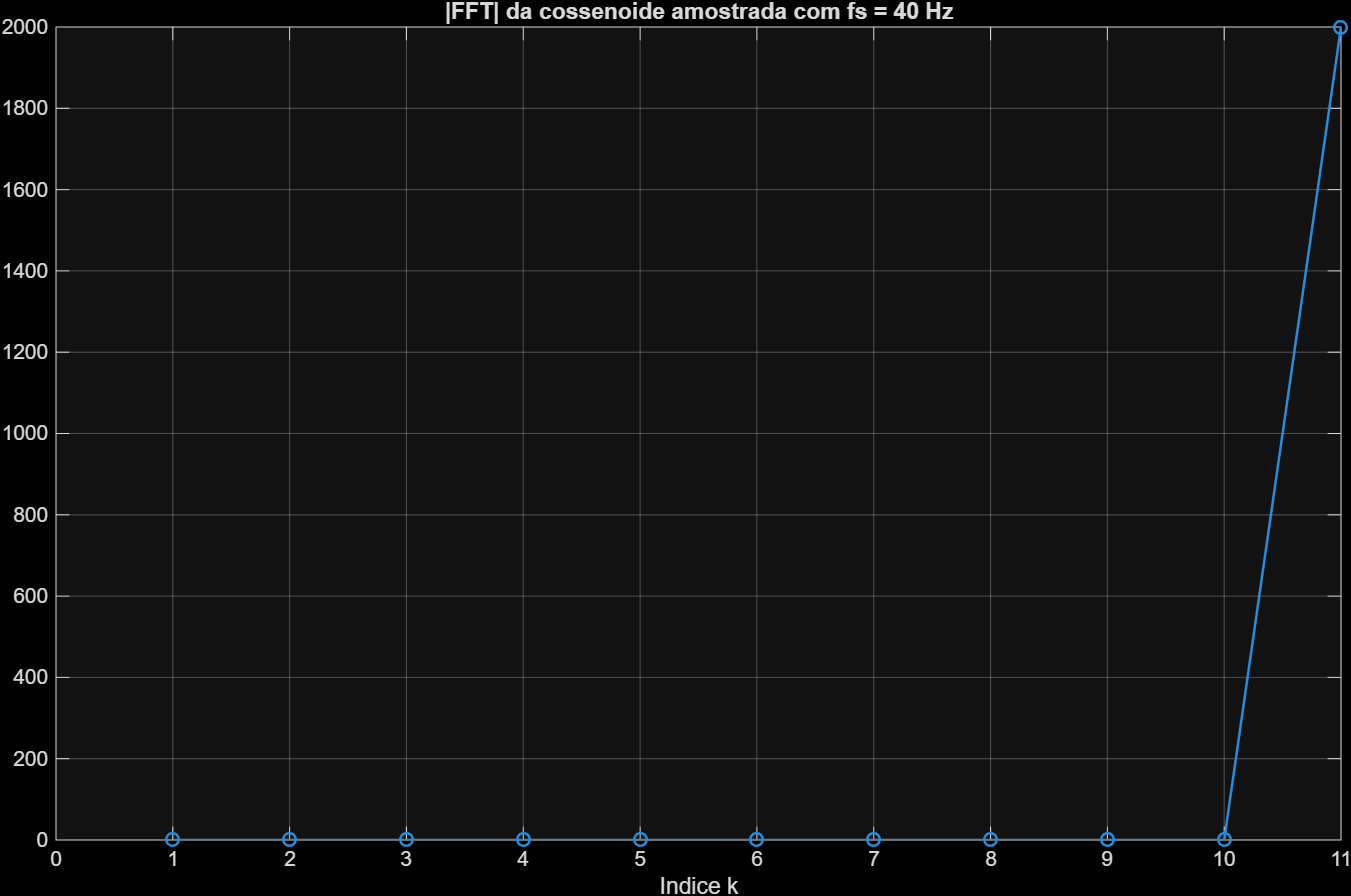
\includegraphics[width=0.85\textwidth]{imgs/q3_cos_40_fft.png}
    \caption{Cossenoide 10\,Hz amostrada a $f_s = 40$\,Hz - $|\text{FFT}|$ até $k=11$.}
\end{figure}

\subsection{Batimento na cossenoide com $f_s = 20{,}01$\,Hz (4000 amostras)}

\begin{figure}[H]
    \centering
    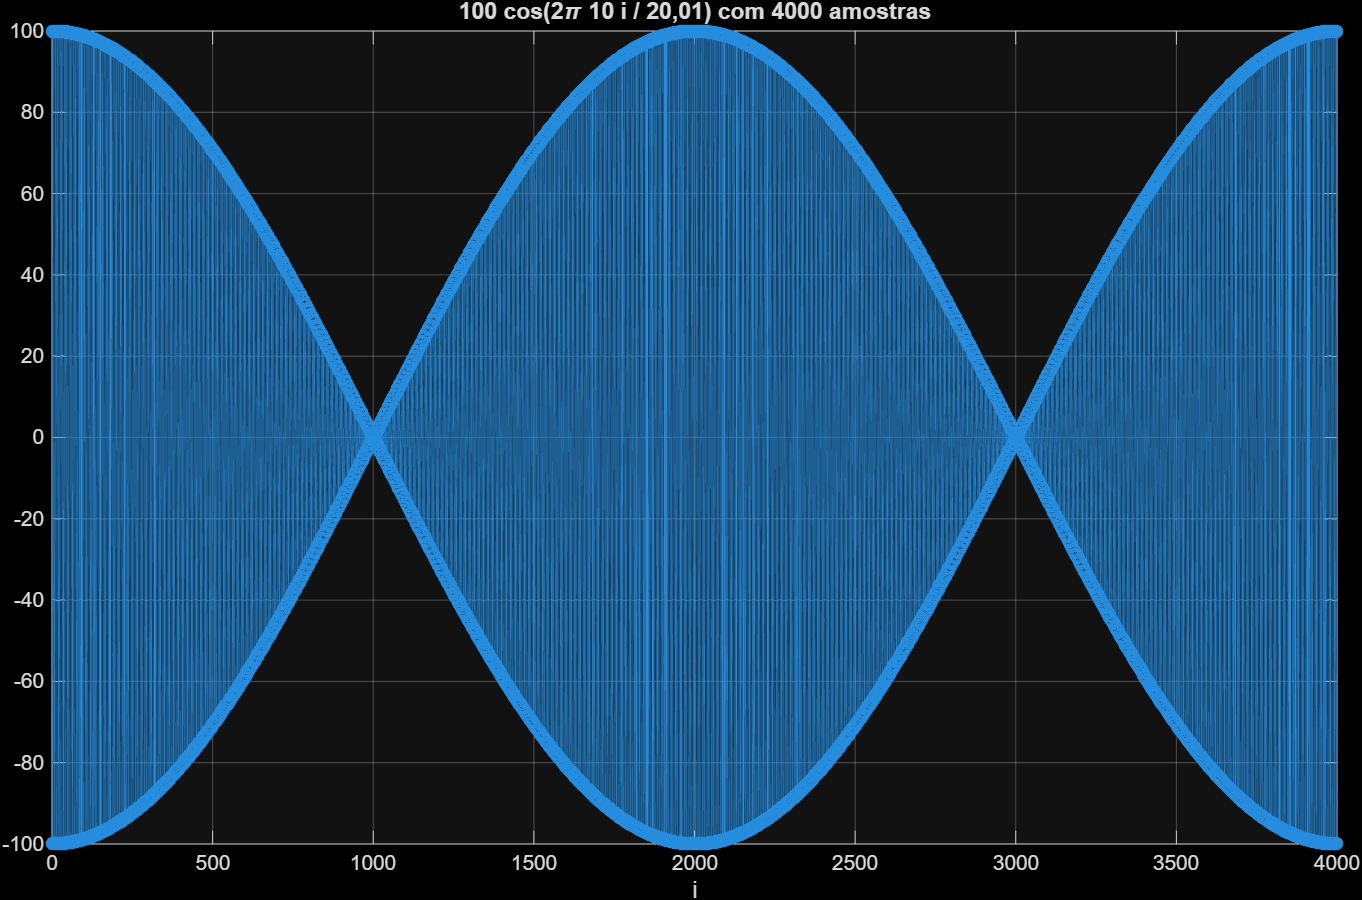
\includegraphics[width=0.85\textwidth]{imgs/q3_batimento_cos_2001.png}
    \caption{$100\cos(2\pi\cdot 10\cdot i/20{,}01)$ com 4000 amostras.}
\end{figure}

\subsection{Conclusões}

A análise quanto a aliasing/recuperação é \textbf{idêntica} à da senoide para todas as frequências de amostragem testadas — o critério de Nyquist depende apenas das frequências $f$ e $f_s$, não da fase do sinal. As mesmas raias aparecem nas mesmas posições $k$ da FFT, e a fronteira aliasing/recuperação ocorre exatamente no mesmo $f_s = 20$\,Hz.

\textbf{O que muda é a forma da reconstrução:}
\begin{itemize}
    \item Em $f_s = 5$\,Hz a cossenoide produz amostras dominadas pela componente de DC (cossenoide amostrada sempre em $\theta = 0, 4\pi, 8\pi, \ldots$, todas com valor próximo de $+100$), enquanto a senoide produzia uma rampa próxima de zero. A FFT da cossenoide tem energia significativa em $k=1$ (componente DC, amplitude 500), enquanto a senoide tem componente DC nula.
    \item Em $f_s = 20$\,Hz, a senoide amostrada nos zeros pode ficar identicamente nula; já a cossenoide, amostrada nos picos $\pm 100$, produz uma onda quadrada alternada — ambas ``corretas'' do ponto de vista espectral mas com formas temporais diametralmente diferentes.
    \item Para os demais $f_s$, ambas as reconstruções convergem visualmente para a forma esperada à medida que $f_s$ cresce, com a única diferença sendo o deslocamento de fase entre a versão amostrada e a contínua.
\end{itemize}

A lição é importante: \emph{o teorema de Nyquist garante apenas a unicidade da reconstrução, não a sua aparência visual em janelas curtas}. Para fins de análise espectral as duas formas de onda são equivalentes; para fins de display ou de processamento que dependa da forma temporal exata (ex.: detecção de picos), a fase relativa entre o sinal e a grade de amostragem é tão importante quanto a frequência de amostragem.

\clearpage
\section{Interpolação de sinais. Aumento da taxa de amostragem após o sinal já ter sido adquirido}

A ideia da interpolação no domínio da frequência é levar o sinal à DFT, preencher com zeros (\textit{zero-padding} no espectro) para ``esticar'' o eixo de frequências e voltar para o tempo via IDFT — obtendo mais amostras por segundo do mesmo sinal sem precisar reamostrar fisicamente.

\subsection{Sinal sem aliasing}

\begin{lstlisting}
figure(30)
for n = 1:100
    x(n) = sin(2*pi*5*(n-1)/100);
end
energ_x = sum(x.*x) % energia = somatorio(sinal)^2 = 50

subplot(3,2,1); plot(x, '.-'); title('sinal original sem aliasing');

dftx = DFT(x); % dftx(6) = 50
subplot(3,2,2); plot(abs(dftx)); axis([0 10 -2 60]);
title('abs da DFT do sinal original');

dftx(51:200) = complex(0,0);
y = IDFT(dftx);
energ_y = sum(y.*y) % 12,5 = 50/4 (4x maior em comprimento)

subplot(3,2,3); plot(abs(dftx)); axis([0 10 -2 60]);
title('DFT com zeros (corte em k=10)');

subplot(3,2,4); plot(y, '.-');
title('sinal reconstituido (mudanca na amplitude)');

dftx2 = 4*dftx; % vezes 4 para amplitude = 1
subplot(3,2,5); plot(abs(dftx2)); axis([0 10 -8 240]);
title('DFT preenchida com zeros e x4');

ynew = IDFT(dftx2);
subplot(3,2,6); plot(ynew, '.-');
title('sinal reconstituido (com correcao da amplitude)');
energ_ynew = sum(ynew.*ynew) % 200
\end{lstlisting}

\begin{figure}[H]
    \centering
    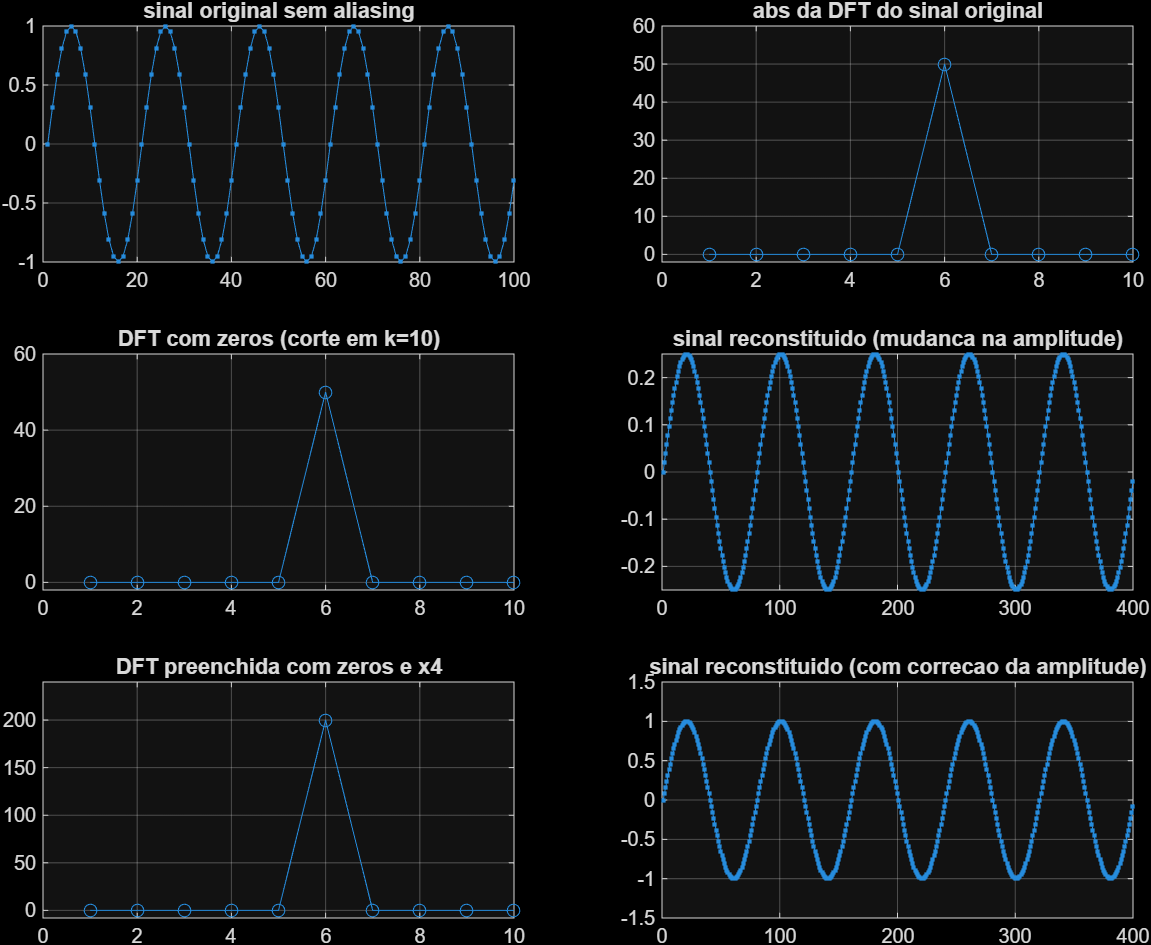
\includegraphics[width=0.95\textwidth]{imgs/q4_sem_aliasing.png}
    \caption{Resultados sem aliasing: sinal original, DFT, DFT preenchida com zeros, sinal reconstruído (com perda e com correção de amplitude). Os subplots de $|\text{FFT}|$ foram cortados em $k=10$, logo após o pico em $k=6$.}
\end{figure}

\textbf{Por que multiplicar a DFT por 4?} O sinal original tem 100 amostras. A senoide $\sin(2\pi\cdot 5(n-1)/100)$ tem amplitude $A=1$ e completa exatamente 5 ciclos no intervalo (cai em $k=6$ na convenção 1-indexed). Na DFT da implementação utilizada, $|\mathrm{DFT}(x)|_{\max} = A\cdot N/2 = 1\cdot 100/2 = 50$. Isso é confirmado por \texttt{energ\_x = 50}, conforme o teorema de Parseval.

Ao preencher o espectro de 100 para 200 pontos (com zeros nos índices 51 a 200) e aplicar a IDFT, esta implementação reconstrói $400$ amostras no tempo (o tamanho da DFT preenchida representa a metade do espectro completo simétrico). Para manter $A=1$ no novo sinal de $N'=400$ amostras é preciso $|\mathrm{DFT}|_{\max} = N'/2 = 200$, ou seja, $200/50 = 4$ vezes o valor original. Em termos energéticos: a energia cresce proporcionalmente ao número de amostras ($50 \to 200 = 4\cdot 50$), exatamente o fator de aumento de comprimento.

Sem a correção, a IDFT devolve um sinal com a mesma forma mas com amplitude $1/4$ e energia $50/4 = 12{,}5$, justamente os valores impressos por \texttt{energ\_y}. Com a correção (\texttt{dftx2 = 4*dftx}), o sinal reconstruído \texttt{ynew} tem amplitude $1$ e energia $200$, conforme esperado.

\subsection{Sinal com aliasing}

\begin{lstlisting}
figure(31)
for n = 1:500
    xo(n) = sin(2*pi*95*(n-1)/500); % sinal "original" 95Hz
end
indice1 = 1:5:500;
for n = 1:100
    x(n) = sin(2*pi*95*(n-1)/100); % com aliasing -> aparenta 5Hz
end

subplot(3,2,1);
plot(xo, '-r'); hold on;
plot(indice1, x, '.-b');
title('original 95Hz (vermelho), com aliasing 5Hz (azul)');

dftx = DFT(x);
subplot(3,2,2); plot(abs(dftx)); axis([0 10 -2 60]);
title('abs da DFT do sinal amostrado');

dftx(51:200) = 0+0i;
y = IDFT(dftx);

subplot(3,2,3); plot(abs(dftx)); axis([0 10 -2 60]);
title('DFT com zeros (corte em k=10)');

subplot(3,2,4); plot(y, '.-');
title('reconstruido (inversao de fase, amplitude)');

subplot(3,2,6); plot(abs(DFT(y))); xlim([0 10]);
title('DFT do sinal reconstituido');
\end{lstlisting}

\begin{figure}[H]
    \centering
    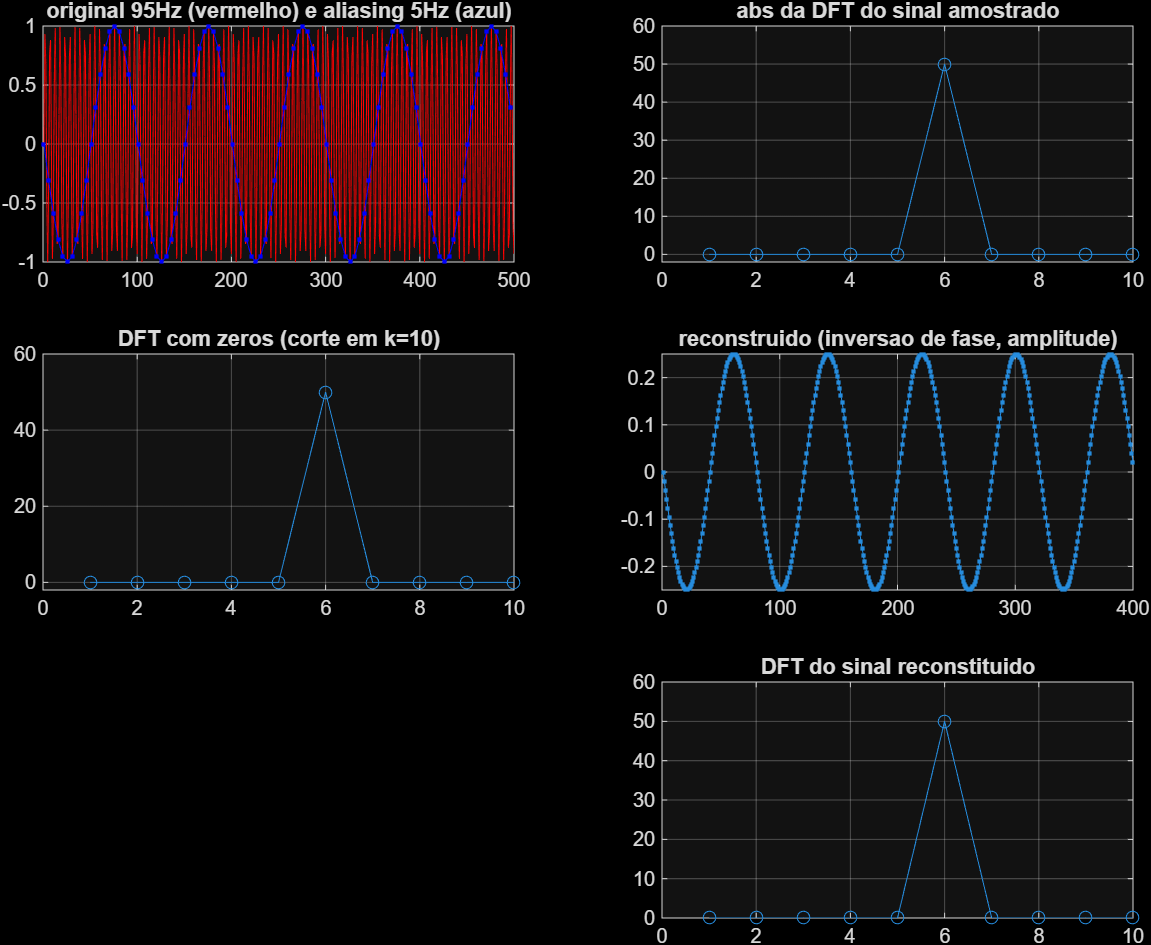
\includegraphics[width=0.95\textwidth]{imgs/q4_com_aliasing.png}
    \caption{Resultados com aliasing: o sinal original de 95\,Hz (vermelho) é amostrado abaixo de Nyquist e aparece como uma senoide de 5\,Hz (azul). A reconstrução via interpolação no espectro recupera os 5\,Hz \emph{aparentes} (com inversão de fase devida ao espelhamento $f_s - f$), e nunca os 95\,Hz originais. Os subplots de $|\text{FFT}|$ foram cortados em $k=10$, logo após o pico em $k=6$.}
\end{figure}

\subsection{Análise: explique o que foi feito no item 4}

A interpolação por zero-padding na DFT é uma operação realizada no espectro \emph{já amostrado}. Como tal, ela não pode inventar componentes que foram destruídas (espelhadas) pelo aliasing. O que vemos no resultado confirma exatamente isso:

\begin{itemize}
    \item \textbf{Sem aliasing:} o sinal de 5\,Hz amostrado em 100 pontos com $f_s = 100$\,Hz tem espectro concentrado em $k=6$ (= $5\cdot 100/100 + 1$). A interpolação dobra o tamanho da DFT (51 $\to$ 200), e a IDFT com correção de amplitude $\times 4$ devolve uma senoide com 400 amostras de mesma amplitude $A=1$ e mesma frequência (5\,Hz) — exatamente como se o sinal tivesse sido amostrado a $f_s = 400$\,Hz desde o início.

    \item \textbf{Com aliasing:} o sinal de 95\,Hz amostrado em $f_s=100$\,Hz tem $f_s/2 = 50$\,Hz $<$ 95\,Hz, violando Nyquist. A componente real de 95\,Hz é refletida em torno de $f_s/2$ e aparece em $|f_s - f| = 5$\,Hz, com uma inversão de sinal. A DFT do sinal amostrado mostra um pico em $k=6$ (= $5\cdot 100/100 + 1$), \emph{indistinguível} de um sinal real de 5\,Hz amostrado a 100\,Hz. A interpolação espectral preserva esse pico e faz a IDFT, gerando um sinal de 5\,Hz interpolado em 400 pontos. Como a interpolação é matematicamente correta a partir do espectro disponível, o sinal de 5\,Hz interpolado coincide com a versão alias original (mostrada em azul nos pontos amostrados), mas é completamente diferente do sinal verdadeiro de 95\,Hz (vermelho). Há também a inversão de fase observável no tempo, decorrente da reflexão $f \to f_s - f$.
\end{itemize}

Isto confirma que \textbf{a interpolação no espectro é útil somente quando o sinal original foi adequadamente amostrado} (acima de Nyquist). Caso contrário, o que se interpola é o conteúdo \emph{aparente} do espectro alias, sem qualquer relação com o sinal físico original. Reforça a importância de filtros anti-aliasing analógicos antes da conversão A/D em sistemas reais — uma vez ocorrido o aliasing, nenhum processamento posterior consegue desfazê-lo.

\clearpage
\section{Conclusão Final}

A prática integrou três conceitos centrais e interdependentes em sistemas lineares discretos: \emph{quantização}, \emph{amostragem} e \emph{interpolação espectral}. Os experimentos realizados permitem extrair as seguintes conclusões consolidadas.

\paragraph{Quantização (item 1).} O erro de quantização decai exponencialmente com o número de bits ($\Delta = 2^{8-M}$), de modo que cada bit adicional reduz o erro máximo pela metade e aumenta a SQNR em aproximadamente $6$\,dB. A passagem de 2 para 5 bits utilizada no experimento traz um ganho de $\approx 18$\,dB e torna o degrau visualmente quase indistinguível do sinal amostrado. Tão importante quanto o número de bits é o \emph{método de arredondamento}: o \texttt{floor} introduz \textit{bias} sistemático negativo de até $-\Delta$ (ou $-\Delta/2$ na média), enquanto o \texttt{round} distribui o erro simetricamente, preserva a média do sinal e reduz a magnitude máxima do erro pela metade — efeito equivalente a quase um bit adicional de resolução. Em projetos práticos, sempre que possível deve-se preferir \texttt{round} (ou truncar com offset de $\Delta/2$, que é matematicamente equivalente).

\paragraph{Amostragem e teorema de Nyquist (itens 2 e 3).} Para um sinal de 10\,Hz, frequências de amostragem $f_s < 20$\,Hz produzem aliasing, com a frequência aparente sendo $|f - f_s|$ ou seu múltiplo mais próximo da banda base. A FFT confirma o deslocamento dos picos: em $f_s=15$ a raia aparece em 5\,Hz, em $f_s=5$ todas as amostras caem em zeros do seno (ou em picos da cossenoide). Apenas com $f_s$ \emph{estritamente} maior que $2f$ a recuperação é possível; o caso $f_s=20{,}01$\,Hz mostra como margens muito pequenas geram \emph{batimentos} de baixa frequência (envelope de $0{,}01$\,Hz, período de 100\,s) que comprometem a reconstrução em janelas curtas. O caso $f_s=20$\,Hz exato é matematicamente o limite, mas falha na prática por depender da fase relativa (uma senoide pode cair toda em zeros e desaparecer, enquanto uma cossenoide cai nos picos e oscila $\pm 100$). A regra prática é trabalhar com $f_s \geq 2{,}5\,f$ para senoides puras e $f_s \geq 5{-}10\,f$ para sinais que precisem ser visualmente reconhecíveis.

\paragraph{Forma de onda (sen vs cos).} A repetição do experimento com cossenoide confirma que \emph{a fase do sinal não altera o critério de Nyquist}: as raias da FFT aparecem nas mesmas posições, a fronteira aliasing/recuperação ocorre no mesmo $f_s$. A diferença observável fica restrita à \emph{forma temporal} dos sinais reconstruídos — particularmente nítida nos casos de aliasing severo, onde a cossenoide amostrada em $f_s = 5$\,Hz resulta em uma sequência DC enquanto a senoide produz uma sequência de zeros.

\paragraph{Interpolação no espectro (item 4).} O zero-padding na DFT seguido de IDFT aumenta a taxa de amostragem do sinal já adquirido sem alterar seu conteúdo espectral, exigindo apenas correção de amplitude proporcional ao fator de expansão (no caso, $\times 4$ para sair de 100 para 400 amostras). É uma técnica útil para visualização e processamento de sinais bem amostrados, com fundamentação no teorema da amostragem: como a banda do sinal já está limitada a $f_s/2$, a interpolação ideal é justamente a reconstrução de Whittaker-Shannon, que é o que o zero-padding em frequência implementa de maneira eficiente. \emph{No entanto, a interpolação não recupera informação perdida em situações de aliasing}: o experimento com 95\,Hz amostrado a 100\,Hz mostra com clareza que o que se interpola é o sinal alias de 5\,Hz, com inversão de fase, e nunca a componente original de 95\,Hz. Isso reforça a regra de ouro do projeto de sistemas A/D: \textbf{filtre antes de amostrar}, pois nenhum processamento digital posterior consegue desfazer o aliasing.

\paragraph{Síntese.} Em conjunto, os experimentos reforçam que amostragem e quantização precisam ser dimensionadas conforme os requisitos da aplicação ($f_s > 2f_{\max}$ com folga adequada e $M$ compatível com a faixa dinâmica e SQNR desejados), e que técnicas como a interpolação no espectro \emph{complementam} — mas jamais \emph{substituem} — uma aquisição correta. O fluxo correto de projeto é: (i) estabelecer a faixa dinâmica e a frequência máxima do sinal de interesse, (ii) projetar o filtro anti-aliasing analógico, (iii) escolher $f_s$ com folga sobre $2f_{\max}$, (iv) escolher $M$ com base na SQNR alvo, e somente depois (v) aplicar técnicas de processamento como interpolação, decimação, filtragem digital, etc.

\end{document}
